%Version 3.1 December 2024
% See section 11 of the User Manual for version history
%
%%%%%%%%%%%%%%%%%%%%%%%%%%%%%%%%%%%%%%%%%%%%%%%%%%%%%%%%%%%%%%%%%%%%%%
%%                                                                 %%
%% Please do not use \input{...} to include other tex files.       %%
%% Submit your LaTeX manuscript as one .tex document.              %%
%%                                                                 %%
%% All additional figures and files should be attached             %%
%% separately and not embedded in the \TeX\ document itself.       %%
%%                                                                 %%
%%%%%%%%%%%%%%%%%%%%%%%%%%%%%%%%%%%%%%%%%%%%%%%%%%%%%%%%%%%%%%%%%%%%%

\documentclass[pdflatex,sn-vancouver-num]{sn-jnl}% referee option is meant for double line spacing

%%=======================================================%%
%% to print line numbers in the margin use lineno option %%
%%=======================================================%%

%%=========================================================================================%%
%% the documentclass is set to pdflatex as default. You can delete it if not appropriate.  %%
%%=========================================================================================%%

%%Note: the following reference styles support Namedate and Numbered referencing. By default the style follows the most common style. To switch between the options you can add or remove “Numbered” in the optional parenthesis. 
%%The option is available for: sn-basic.bst, sn-chicago.bst%  
 
%%%% Standard Packages
%%<additional latex packages if required can be included here>

\usepackage{graphicx}%
\usepackage{multirow}%
\usepackage{amsmath,amssymb,amsfonts}%
\usepackage{amsthm}%
\usepackage{mathrsfs}%
\usepackage[title]{appendix}%
\usepackage{xcolor}%
\usepackage{textcomp}%
\usepackage{manyfoot}%
\usepackage{booktabs}%
\usepackage{algorithm}%
\usepackage{algorithmicx}%
\usepackage{algpseudocode}%
\usepackage{listings}%
\usepackage{enumitem}%
\usepackage{makecell}%
%%%%

%%%%%=============================================================================%%%%
%%%%  Remarks: This template is provided to aid authors with the preparation
%%%%  of original research articles intended for submission to journals published 
%%%%  by Springer Nature. The guidance has been prepared in partnership with 
%%%%  production teams to conform to Springer Nature technical requirements. 
%%%%  Editorial and presentation requirements differ among journal portfolios and 
%%%%  research disciplines. You may find sections in this template are irrelevant 
%%%%  to your work and are empowered to omit any such section if allowed by the 
%%%%  journal you intend to submit to. The submission guidelines and policies 
%%%%  of the journal take precedence. A detailed User Manual is available in the 
%%%%  template package for technical guidance.
%%%%%=============================================================================%%%%

%% as per the requirement new theorem styles can be included as shown below
\theoremstyle{thmstyleone}%
\newtheorem{theorem}{Theorem}%  meant for continuous numbers
%%\newtheorem{theorem}{Theorem}[section]% meant for sectionwise numbers
%% optional argument [theorem] produces theorem numbering sequence instead of independent numbers for Proposition
\newtheorem{proposition}[theorem]{Proposition}% 
%%\newtheorem{proposition}{Proposition}% to get separate numbers for theorem and proposition etc.

\theoremstyle{thmstyletwo}%
\newtheorem{example}{Example}%
\newtheorem{remark}{Remark}%

\theoremstyle{thmstylethree}%
\newtheorem{definition}{Definition}%

\raggedbottom
%%\unnumbered% uncomment this for unnumbered level heads
\usepackage{bm}
\usepackage{adjustbox}
\usepackage[section]{placeins}

\makeatletter
\renewenvironment{table}[1][htbp]%
{\begin{tableorg}[#1]%
\begin{center}
\begin{adjustbox}{max width=\linewidth}
\begin{threeparttable}
\tablebodyfont%
\renewcommand\footnotetext[2][]{{\removelastskip\vskip3pt%
\let\tablebodyfont\tablefootnotefont%
\hskip0pt\if!##1!\else{\smash{$^{##1}$}}\fi##2\par}}%
}{\end{threeparttable}\end{adjustbox}\end{center}\end{tableorg}}
\makeatother

\makeatletter
\def\mycline#1{\@mycline#1\@nil}
\def\@mycline#1-#2\@nil{%
  \omit
  \@multicnt#1%
  \advance\@multispan\m@ne
  \ifnum\@multicnt=\@ne\@firstofone{&\omit}\fi
  \@multicnt#2%
  \advance\@multicnt-#1%
  \advance\@multispan\@ne
  \leaders\hrule\@height\arrayrulewidth\hfill
  \cr
  \noalign{\vskip-\arrayrulewidth}}
\makeatother
\begin{document}

\title[Flexi-JEGNN]{Flexi-JEGNN: A Probe for Geometric Sensitivity in Bioactivity Prediction}

%%=============================================================%%
%% GivenName	-> \fnm{Joergen W.}
%% Particle	-> \spfx{van der} -> surname prefix
%% FamilyName	-> \sur{Ploeg}
%% Suffix	-> \sfx{IV}
%% 
\author[1]{\fnm{Nethravathi} \sur{B}}\email{nethravathi.sai@gmail.com}
\author*[2]{\fnm{Pooja} \sur{Gupta}}\email{pooja.gupta@jaipur.manipal.edu}
\author[1]{\fnm{Manoj M.} \sur{Krishna}}\email{manojmk2k80@gmail.com}
\author[1]{\fnm{Parnika} \sur{Madhukumar}}\email{parnikamadhukumarr@gmail.com}
\author[1]{\fnm{Vedika} \sur{Lakshmisha}}\email{vedikalakshmisha@gmail.com}
\author[1]{\fnm{Abhinav} \sur{Trivedi}}\email{abhinavcanbecontacted@gmail.com}

\affil[1]{\orgdiv{Department of Information Science and Engineering}, \orgname{JSS Academy of Technical Education}, \orgaddress{\city{Bengaluru}, \country{India}}}
\affil[2]{\orgdiv{Department of Data Science and Engineering}, \orgname{Manipal University Jaipur}, \orgaddress{\city{Jaipur}, \country{India}}}

%%==================================%%
%% Sample for unstructured abstract %%
%%==================================%%

\abstract{This paper presents \textbf{Flexi-JEGNN}, a controlled probe isolating the predictive contribution of geometric precision \emph{within the scalar-distance message-passing paradigm}. By accepting five distance levels--a constant scalar to a true 3D conformer--without architectural modification, the model varies only the edge distance $e_{ij}$ while holding all other factors constant. Across 3,250 training runs on six benchmarks ($n{=}20$ seeds), a one-way ANOVA over physically meaningful levels (L0--L3) is non-significant ($p{=}0.070$--$0.549$). With Cohen's $f$ at or below the small-effect threshold and Bayes Factors ($\mathrm{BF}_{01}=84.6$--$631.1$) providing evidence for the null on five of six benchmarks, this pattern is reproduced across SchNet, DimeNet, and Uni-Mol, with topology-only models (D-MPNN, GIN, Random Forest) bounding the comparison. As no statistically detectable advantage of higher geometric fidelity is observed—even for protein–ligand affinity regression—these results support 2D topological encodings as the Pareto-efficient choice for virtual screening. These conclusions are limited to scalar distance models and MoleculeNet/TDC benchmark distributions; evaluating equivariant architectures (EGNN, PaiNN) and geometry-sensitive benchmarks remains the critical next test.}

\keywords{Graph Neural Networks, Molecular Representation Learning, Drug Discovery, Geometric Deep Learning, Virtual Screening}

%%\pacs[JEL Classification]{D8, H51}

%%\pacs[MSC Classification]{35A01, 65L10, 65L12, 65L20, 65L70}

\maketitle

\section{Introduction}
\label{sec:intro}

Rapid scoring of large molecular libraries for bioactivity is a central
bottleneck in computational drug discovery.  Graph Neural Networks (GNNs)
have emerged as the leading paradigm: they operate directly on molecular
graphs, are permutation-invariant by construction, and achieve
$\mathcal{O}(N{+}E)$ inference from SMILES strings alone
\cite{zhang2025,kipf2017gcn,gilmer2017mpnn}.  Foundational architectures showed that
atom-level features propagated through bond connectivity suffice to learn
chemically meaningful representations \cite{duvenaud2015fingerprints};
directed messaging \cite{yang2019dmpnn} and graph attention subsequently improved expressivity.

A second generation of architectures argued that these topological models
miss through-space interactions governing biological activity and introduced
explicit 3D atomic coordinates.  SchNet \cite{schutt2018schnet} introduced
continuous radial filters over pairwise Euclidean distances; DimeNet
\cite{klicpera2020dimenet} added angular features; and large pre-trained
models such as GEM \cite{fang2022gem} and Uni-Mol \cite{zhou2023unimol}
pre-train on millions of 3D conformations.  These architectures achieve
strong benchmark scores, but at a steep cost: generating a single 3D
conformer via ETKDGv3 \cite{riniker2015etkdg} requires $\mathcal{O}(N^3)$
\cite{Wang2026} distance geometry plus force-field minimisation
\cite{tosco2014mmff}.  For virtual libraries containing billions of
compounds---ZINC-22 alone enumerates over 4.5 billion purchasable molecules, and databases such as ChEMBL \cite{gaulton2012chembl} aggregate millions of bioactivity records---this overhead
is a fundamental scalability barrier.

The assumption underlying this investment---that 3D geometry provides
irreplaceable predictive signal---has been empirically challenged by
\cite{praski2025benchmarking}, which used hierarchical Bayesian testing to
show that highly parameterised 3D models frequently produce negligible
improvement over 2D fingerprint baselines.  But that study compared
\emph{architecturally different} models, conflating the effect of 3D
geometry with architectural capacity.  The core causal question remains
open: does spatial geometry \emph{itself} provide predictive signal on
these tasks?

This paper answers that question through a controlled threshold experiment.
Flexi-JEGNN is presented here as a controlled probe framework whose
defining property is the ability to ingest any of five distance
representation levels without modification.  All other
factors---layer count, hidden dimensionality, aggregation, optimiser,
dataset splits---are held constant, producing a clean causal estimate of
geometric precision's contribution to predictive performance.

\noindent\textbf{Null hypothesis (H$_0$).}
\emph{Restricting attention to physically meaningful distance
representations (L0--L3), there is no statistically significant difference
in mean predictive performance across any pair of distance levels on any of
the six benchmarks evaluated.}

\noindent\textbf{Alternative hypothesis (H$_1$).}
\emph{Higher-fidelity 3D geometric distance representations (L2, L3) provide statistically significant improvements in predictive performance over pure 2D topological representations (L0, L1).}
Rejection of the null would be required
to justify $\mathcal{O}(N^3)$ conformer generation for standard bioactivity
screening.

\noindent\textbf{Scope of claims.}  The probe varies a single scalar edge
distance and therefore tests geometric sensitivity \emph{within the
scalar-distance (rotation-invariant) message-passing paradigm}.  All
conclusions below are stated for that paradigm and for the MoleculeNet/TDC
benchmark distributions evaluated.  Equivariant architectures (EGNN,
PaiNN), whose coordinate-update and vector-feature mechanisms exploit
geometry through fundamentally different primitives, are explicitly out of
scope: they cannot be driven by a scalar-distance level without altering
the architecture, which would break the controlled comparison
(Section~\ref{ssec:summary_positioning}).  This work does not claim that 3D geometry
is unnecessary for molecular property prediction in general---only that, for
these benchmarks and within this paradigm, finer geometric precision yields
no statistically detectable gain.



\textbf{Summary of Findings.}

Across 3,250 training runs on six benchmarks and six model families,
no statistically significant performance difference is found between
any pair of physically meaningful distance approximations (L0--L3),
including the true 3D conformer level.  The finding holds across all three task
types: bioactivity classification, continuous quantum-chemical regression (QM9, subject to capacity caveats detailed in Section~\ref{sec:limits}),
and protein-ligand affinity regression on the PDBbind 2020 Refined Set---the last with the binding interface held at ground-truth crystal 3D, so only ligand-internal geometric fidelity is varied (Section~\ref{ssec:pdbbind_feat}).  The random null (L4) degrades
performance only on BACE and QM9 (regression), indicating these tasks require
\emph{topological coherence}---not geometric precision.  SchNet, most
closely designed for 3D geometry, shows no consistent benefit from genuine
conformers across the physically meaningful levels on any dataset.  Within the resolution of this study (powered for $f \geq 0.35$; effects observed at $f = 0.07$--$0.12$, with moderate Bayesian evidence for the null), pure 2D approaches (L0/L1) are statistically indistinguishable from the true 3D conformer level on all six benchmarks while requiring zero spatial preprocessing.

\textbf{Contributions.}
\begin{itemize}
  \item \textbf{Flexi-JEGNN}: A flexible joint-edge GNN probe framework that accepts
  any of five distance levels (L0--L4) without architectural modification,
  assembling established components
  (JointEdgeConv adapted from \cite{gasteiger2021synthetic}, PNA readout
  from \cite{corso2020pna}, Gaussian smearing from \cite{schutt2018schnet})
  into a controllable within-architecture ablation apparatus for geometric
  sensitivity analysis.

  \item \textbf{Extended threshold experiment} ($n{=}20$ seeds,
  6 datasets, 6 model families): Restricted ANOVA yields $p > 0.05$ on every
  dataset across classification and regression tasks alike, with Bayes
  Factors giving moderate evidence for the null on five of six benchmarks.
  BACE and QM9 require topological coherence. Neither through-space connectivity nor distance precision individually yields a statistically detectable benefit that would justify the $\mathcal{O}(N^3)$ cost.

  \item \textbf{Insensitivity reproduced across model families}: Of the comparative models, SchNet, DimeNet and Uni-Mol accept the full L0--L4 range; across the physically meaningful levels (L1--L3), all show the same insensitivity as the probe, while the topology-only baselines (D-MPNN, GIN, Random Forest) bound the comparison.  A single anomaly is reported transparently (Uni-Mol on QM9 at L4) alongside a mechanistic exception (the L0 collapse of radial-basis models), neither of which overturns the within-model null.
  Additionally, the performance collapse at L0 reveals a mechanistic vulnerability in RBF-based architectures when spatial diversity is absent, defining their minimum operating condition.

  \item \textbf{Cost-dominant 2D frontier}: L0/L1 (zero spatial cost) is statistically indistinguishable from
  L2/L3 on all six benchmarks, making them the cost-dominant (Pareto-efficient)
  choice for virtual screening on standard MoleculeNet/TDC bioactivity benchmarks within the resolution of this study.

  \item \textbf{Benchmark critique}: Quantitative evidence that MoleculeNet
  bioactivity benchmarks do not expose the geometric sensitivity needed to
  evaluate 3D GNN architectures.
\end{itemize}

\subsection*{Paper Organisation} The remainder of the paper is organised as follows:
Section~\ref{sec:related} reviews related work in topological and geometric molecular representations.
Section~\ref{sec:methods} details the Flexi-JEGNN architecture, distance levels, and experimental protocol.
Section~\ref{sec:results} presents the empirical results across six benchmarks.
Section~\ref{sec:discussion} interprets the mechanistic and practical implications.
Section~\ref{sec:limits} outlines limitations. Section~\ref{sec:conclusion_future} discusses future directions and concludes.
\section{Related Work}
\label{sec:related}

\subsection{2D Message-Passing Foundations}

Kipf and Welling's GCNs \cite{kipf2017gcn} and Gilmer \emph{et al.}'s
MPNN framework \cite{gilmer2017mpnn} established iterative neighbourhood
aggregation as the standard paradigm for molecular property prediction.
D-MPNN \cite{yang2019dmpnn} introduced directed bond-level messaging and
demonstrated that learned molecular representations can match or outperform
fixed descriptor models on specific benchmarks, though empirical studies
have noted that a clear winner has yet to emerge across all chemical
spaces~\cite{yang2019dmpnn}.
These models require no spatial preprocessing, and
Chemprop~v2 \cite{graff2026chempropv2} has since optimised the D-MPNN
family further, achieving a 2$\times$ speedup and 3$\times$ memory
reduction while maintaining competitive screening accuracy.

\subsection{3D Geometric Deep Learning}

The realisation that molecular bioactivity is governed by 3D
through-space interactions motivated a second generation of architectures.
SchNet \cite{schutt2018schnet} introduced continuous radial filters over
pairwise Euclidean distances; DimeNet \cite{klicpera2020dimenet} and
GemNet \cite{gasteiger2021gemnet} extended this with angular and torsional features.  Large
pre-trained models pushed expressiveness further: GEM \cite{fang2022gem}
embedded 3D spatial primitives directly into pre-training; Uni-Mol
\cite{zhou2023unimol} and GROVER \cite{rong2020grover} pre-trained on
millions of conformers; and Uni-Mol$+$ \cite{lu2024unimolplus} employed
a two-track Transformer that iteratively refines RDKit conformations
toward DFT equilibrium, demonstrating that conformation quality is
paramount for quantum chemical properties.  More recent architectures
such as OmniMol \cite{wang2025omnimol}, which uses an SE-equivariant
hypergraph with a task-agnostic Mixture-of-Experts backbone, and
Platonic Transformers \cite{islam2025platonictransformerssolidchoice},
which process molecules as rigid 3D solids, continue to push
state-of-the-art on energy and force benchmarks.

Despite their expressiveness, 3D models frequently fail to outperform 2D
baselines on standard bioactivity tasks \cite{praski2025benchmarking}.
Yang \emph{et al.}\ \cite{yang2019dmpnn} further found that 3D GNN
gains are highly task- and split-dependent, with no modelling class
yet demonstrating universal dominance when generalising to new chemical
spaces.  Novel architectures such as
Kolmogorov--Arnold GNNs \cite{kangnn2025} and Stereoelectronics-Infused
Molecular Graphs \cite{Boiko_2025} have demonstrated strong property
prediction without relying on true 3D coordinates, the latter by
injecting chemical physics directly into 2D graph structure.  Quantized
GNNs \cite{rasool2025quantized} pursue efficiency from a hardware angle,
showing that reduced-precision inference preserves accuracy for
high-throughput deployment.

\subsection{The Conformer Crisis and Efficiency Trade-offs}

A growing body of evidence points to a ``conformer crisis'': 3D models
only consistently outperform 2D baselines when given access to
ground-truth or near-equilibrium conformers.  Hamakawa and Miyao
\cite{hamakawa2025conformation} showed that lower-quality RDKit
conformers frequently cause 3D models to underperform standard 2D
fingerprints.  Castañeda-Leautaud and Amaro \cite{Castaneda_Leautaud_2025}
demonstrated that simpler attentive spatial models can be 2.3$\times$
faster than 3D optimisation-based methods while delivering comparable
bioactivity metrics, suggesting diminishing returns from equivariant
complexity.  Table~\ref{tab:approx_quality} in Section~\ref{sec:results}
quantifies this trade-off concretely, showing up to a 159$\times$
slowdown for ETKDGv3 relative to the simplest baseline.

\subsection{Pre-training, Information Fusion, and Multi-Conformer Methods}

To avoid the inference-time cost of 3D coordinates, several approaches
transfer geometric knowledge into 2D models during pre-training.
3D~Infomax \cite{stark2022infomax} maximises mutual information between
2D graph and 3D conformer representations, allowing a 2D model to
``inherit'' 3D knowledge without requiring coordinates at test time---a
finding consistent with the finding that explicit 3D coordinates add no
incremental value on bioactivity benchmarks.  GeoRecon
\cite{yan2025georecongraphlevelrepresentationlearning} extends this idea
with a reconstruction-based pre-training objective.  ConforFormer
\cite{klein2026conforformer} instead leverages multi-conformer ensembles
at training time for improved stability across diverse scaffolds; whether
ensemble representations expose geometric sensitivity not seen in
single-conformer experiments remains an open question addressed in
Section~\ref{sec:limits}.

\subsection{Synthetic Coordinates and the Gasteiger Prior Art}
\label{ssec:gasteiger}

The idea of deriving approximate spatial information from molecular
topology was introduced by Gasteiger \emph{et al.}\
\cite{gasteiger2021synthetic} (NeurIPS 2021), who proposed distance
geometry bounds and Personalised PageRank as synthetic coordinates for
\emph{directional} MPNNs, achieving a 55\% error reduction on ZINC and
matching ETKDGv3 on QM9.  \textbf{Flexi-JEGNN differs in three
respects}: (i)~it uses a \emph{non-directional} MPNN that treats
distances as joint edge scalars rather than angular directional features;
(ii)~it targets \emph{macroscopic bioactivity classification}; and
(iii)~it is used as a \emph{controlled probe} spanning all five distance
levels rather than as a replacement for missing 3D data.  The L2
distance geometry midpoint is explicitly adapted from Gasteiger
\emph{et al.}\ and is acknowledged as prior art, not a novel
contribution.

Multi-aggregation pooling was formalised by Corso \emph{et al.}\
\cite{corso2020pna}, proving that sum, mean, and max aggregators jointly
are required to uniformly approximate continuous feature domains.
Flexi-JEGNN's readout builds directly on this result.

\subsection{Benchmark Design}

Deng \emph{et al.}\ \cite{deng2023systematic} showed that Murcko scaffold
splits better reflect real-world scaffold generalisation; the authors
adopt them throughout.  Stärk \emph{et al.}\ \cite{stark2022infomax}
showed that 3D geometric information transfers to 2D models implicitly,
consistent with the observation that explicit 3D coordinates add no
incremental value on bioactivity tasks.  Table~\ref{tab:lit_comparison}
summarises how Flexi-JEGNN relates to the architectures discussed above.

The work most directly relevant to the present paper is Praski \emph{et al.}~\cite{praski2025benchmarking}, which applied hierarchical Bayesian testing to show that heavily parameterised 3D models frequently deliver negligible accuracy gains over 2D fingerprint baselines.  That result is significant and complementary, but it leaves open a fundamental causal question: because the compared models differ not only in their use of 3D coordinates but also in architecture, capacity, and pre-training regime, any observed performance gap (or lack thereof) could be attributed to modelling differences rather than to the geometric information itself.  The present work directly addresses this gap.  By holding \emph{all} architectural factors constant and varying only the scalar distance $e_{ij}$, Flexi-JEGNN provides a clean causal estimate of what geometric precision alone contributes.  The finding---no statistically significant difference across L0--L3 on any of six benchmarks---converges with and strengthens that conclusion, while supplying the architectural-control mechanism that study could not provide.  A further distinction is task coverage: the present study expands beyond classification to include quantum-chemical regression (QM9) and protein-ligand affinity regression on the PDBbind 2020 Refined Set, demonstrating that geometric insensitivity holds across all three task types.


\begin{table}[htbp]
  \centering
  \caption{Comparative analysis of recent molecular representation architectures and their distinction from the proposed Flexi-JEGNN framework.}
  \label{tab:lit_comparison}
  \renewcommand{\arraystretch}{1.1} 
  \setlength{\tabcolsep}{4pt}
  \scriptsize 
  \begin{tabular}{|p{0.14\textwidth}|p{0.21\textwidth}|p{0.21\textwidth}|p{0.18\textwidth}|p{0.19\textwidth}|}
    \hline
    \textbf{Model (Reference)} & \textbf{Core Methodology} & \textbf{Performance Profile} & \textbf{Computational Efficiency} & \textbf{Distinction from Flexi-JEGNN} \\
    \hline
    
    \textbf{OmniMol} \cite{wang2025omnimol} & SE-equivariant hypergraph with t-MoE backbone. & SOTA in property prediction \& chirality. & \textbf{Low:} Recursive geometry updates. & Focuses on SOTA via complex symmetry. \\
    \hline
    
    \textbf{Chemprop v2} \cite{graff2026chempropv2} & Optimised D-MPNN (2D Graph). & Algorithmic parity with original Chemprop. & \textbf{Very High:} 2$\times$ faster, 3$\times$ less memory. & Purely 2D optimisation; does not probe 2D/3D gap. \\
    \hline
    
    \textbf{KA-GNN} \cite{kangnn2025} & Kolmogorov--Arnold layers in GNNs. & Outperforms conventional GNNs. & \textbf{High:} Improved efficiency over standard GNNs. & Uses mathematical function approximation. \\
    \hline
    
    \textbf{Uni-Mol Analysis} \cite{hamakawa2025conformation} & Benchmarking 2D vs. 3D conformers. & Superior accuracy ONLY with ground-truth. & \textbf{Moderate:} Drops with inaccurate conformers. & Validates premise that noisy 3D underperforms 2D. \\
    \hline
    
    \textbf{Platonic Trans.} \cite{islam2025platonictransformerssolidchoice} & SE-equivariant solid-choice transformer. & High energy/force MAE accuracy. & \textbf{Moderate:} $\sim$2.8ms avg time per molecule. & Targets quantum chemistry where geometry is strict. \\
    \hline
    
    \textbf{Spatial-MP} \cite{Castaneda_Leautaud_2025} & Simple, attentive spatial MPNN. & Comparable metrics between 2D \& 3D. & \textbf{High:} 2.3$\times$ faster than 3D optimisation. & Supports conclusion that 2D is optimal for screening. \\
    \hline
    
    \textbf{ConforFormer} \cite{klein2026conforformer} & Multi-conformer task-agnostic rep. & High stability across diverse conformers. & \textbf{Low:} Requires multiple conformer generations. & Focuses on conformer diversity, not sensitivity. \\
    \hline
    
    \textbf{GeoRecon} \cite{yan2025georecongraphlevelrepresentationlearning} & Graph-level 3D reconstruction pre-training. & Improved performance on QM9 and MD17. & \textbf{Low:} Heavy pre-training/reconstruction costs. & Uses 3D purely for pre-training embeddings. \\
    \hline
    
    \textbf{Quantized GNNs} \cite{rasool2025quantized} & Weight and activation quantization. & Maintains accuracy, reduces model size. & \textbf{Ultra-High:} Focuses on mobile/edge inference. & Efficiency focus is strictly on hardware. \\
    \hline
    
    \textbf{Uni-Mol+} \cite{lu2024unimolplus} & Two-track Transformer with DFT refinement. & High accuracy for quantum chem properties. & \textbf{Very Low:} Iterative refinement to equilibrium. & Assumes high-quality 3D is essential for all tasks. \\
    \hline
    
    \textbf{GEM} \cite{fang2022gem} & Geometry-enhanced pre-training. & Strong benchmarks on MoleculeNet. & \textbf{Moderate:} High cost for 3D pre-training data. & Embeds 3D spatial primitives directly as features. \\
    \hline
    
    \textbf{3D Infomax} \cite{stark2022infomax} & 2D-3D Mutual Information maximisation. & Enhances 2D models for test-time speed. & \textbf{High (Test):} Only uses 2D during inference. & Leverages 3D knowledge exclusively in pre-training. \\
    \hline
    
    \textbf{SIMG} \cite{Boiko_2025} & Stereoelectronics-infused molecular graphs. & Bridges 2D/3D gap for dipole/gaps. & \textbf{High:} Avoids costly DFT calculations. & Injects chemical physics into 2D graphs. \\
    \hline
    
    \textbf{Dir. MPNN} \cite{gasteiger2021synthetic} & Synthetic coordinates via distance bounds. & 55\% error reduction on ZINC. & \textbf{High:} Uses PageRank/Bounds, no conformers. & Replaces missing 3D data rather than evaluating sensitivity. \\
    
    \hline

    \textbf{EGNN} \cite{satorras2021egnn} & $E(n)$-equivariant GNN; updates coordinates and features jointly via relative squared distances. & SOTA on N-body, MD17, QM9 forces. & \textbf{Low:} Dynamic coordinate updates every layer. & Fixed scalar distances (Flexi-JEGNN) vs.\ dynamic equivariant coordinate updates. \\
    \hline

    \textbf{PaiNN} \cite{schutt2021painn} & Equivariant MPNN with vector-valued representations for tensorial property prediction. & SOTA on MD17 and QM9 energy/force. & \textbf{Moderate:} Fixed direction vectors; no position updates. & Rotationally invariant scalars (Flexi-JEGNN) vs.\ rotational equivariance via directional vectors. \\
    \hline
    
  \end{tabular}
\end{table}



%% ===========================================================
\subsection{Summary and Positioning}
\label{ssec:summary_positioning}

Table~\ref{tab:lit_comparison} collects the landscape of recent molecular representation architectures relevant to this work.  Several broad patterns emerge.  First, architectures designed for maximum expressive power on quantum-chemical benchmarks (EGNN, PaiNN, Uni-Mol$+$, Platonic Transformers) do so at the cost of $\mathcal{O}(N^3)$ preprocessing or iterative coordinate refinement, making billion-compound screening infeasible.  Second, efficiency-focused 2D models (Chemprop~v2, KA-GNN, SIMG) demonstrate that strong bioactivity performance is achievable without 3D coordinates, but they do not directly quantify what geometric information \emph{would} contribute if present.  Third, prior probing work (Hamakawa and Miyao \cite{hamakawa2025conformation}; Castañeda-Leautaud and Amaro \cite{Castaneda_Leautaud_2025}; Praski \emph{et al.}\ \cite{praski2025benchmarking}) consistently finds that 3D representations fail to outperform 2D baselines on standard benchmarks, but each study conflates architectural and geometric variation.  Flexi-JEGNN addresses this gap via a controlled within-architecture distance-level ablation that holds all modelling factors fixed, isolating geometric precision as the sole independent variable.  Equivariant architectures (EGNN, PaiNN) were not experimentally tested in this study: while both are included in Table~\ref{tab:lit_comparison} with explicit architectural comparisons against Flexi-JEGNN (symmetry type, coordinate update mechanism, and mathematical basis), their coordinate-update mechanisms---dynamic position updates in EGNN and vector-valued representations in PaiNN---operate on fundamentally different computational primitives than the scalar-distance paradigm used here, making a controlled within-probe comparison infeasible without architectural modification.  The findings below extend to regression settings (QM9, PDBbind) that prior probing work did not cover. \\

\section{Methodology}
\label{sec:methods}


Flexi-JEGNN is designed around a single overriding requirement: the
architecture must accept any of five distance levels without modification to
weights, layers, or hyperparameters.  This is what makes it a
\emph{controlled probe}---the only variable that changes across conditions is
the scalar distance $e_{ij}$ injected at the edge encoding stage.

\begin{figure*}[h]
  \centering
  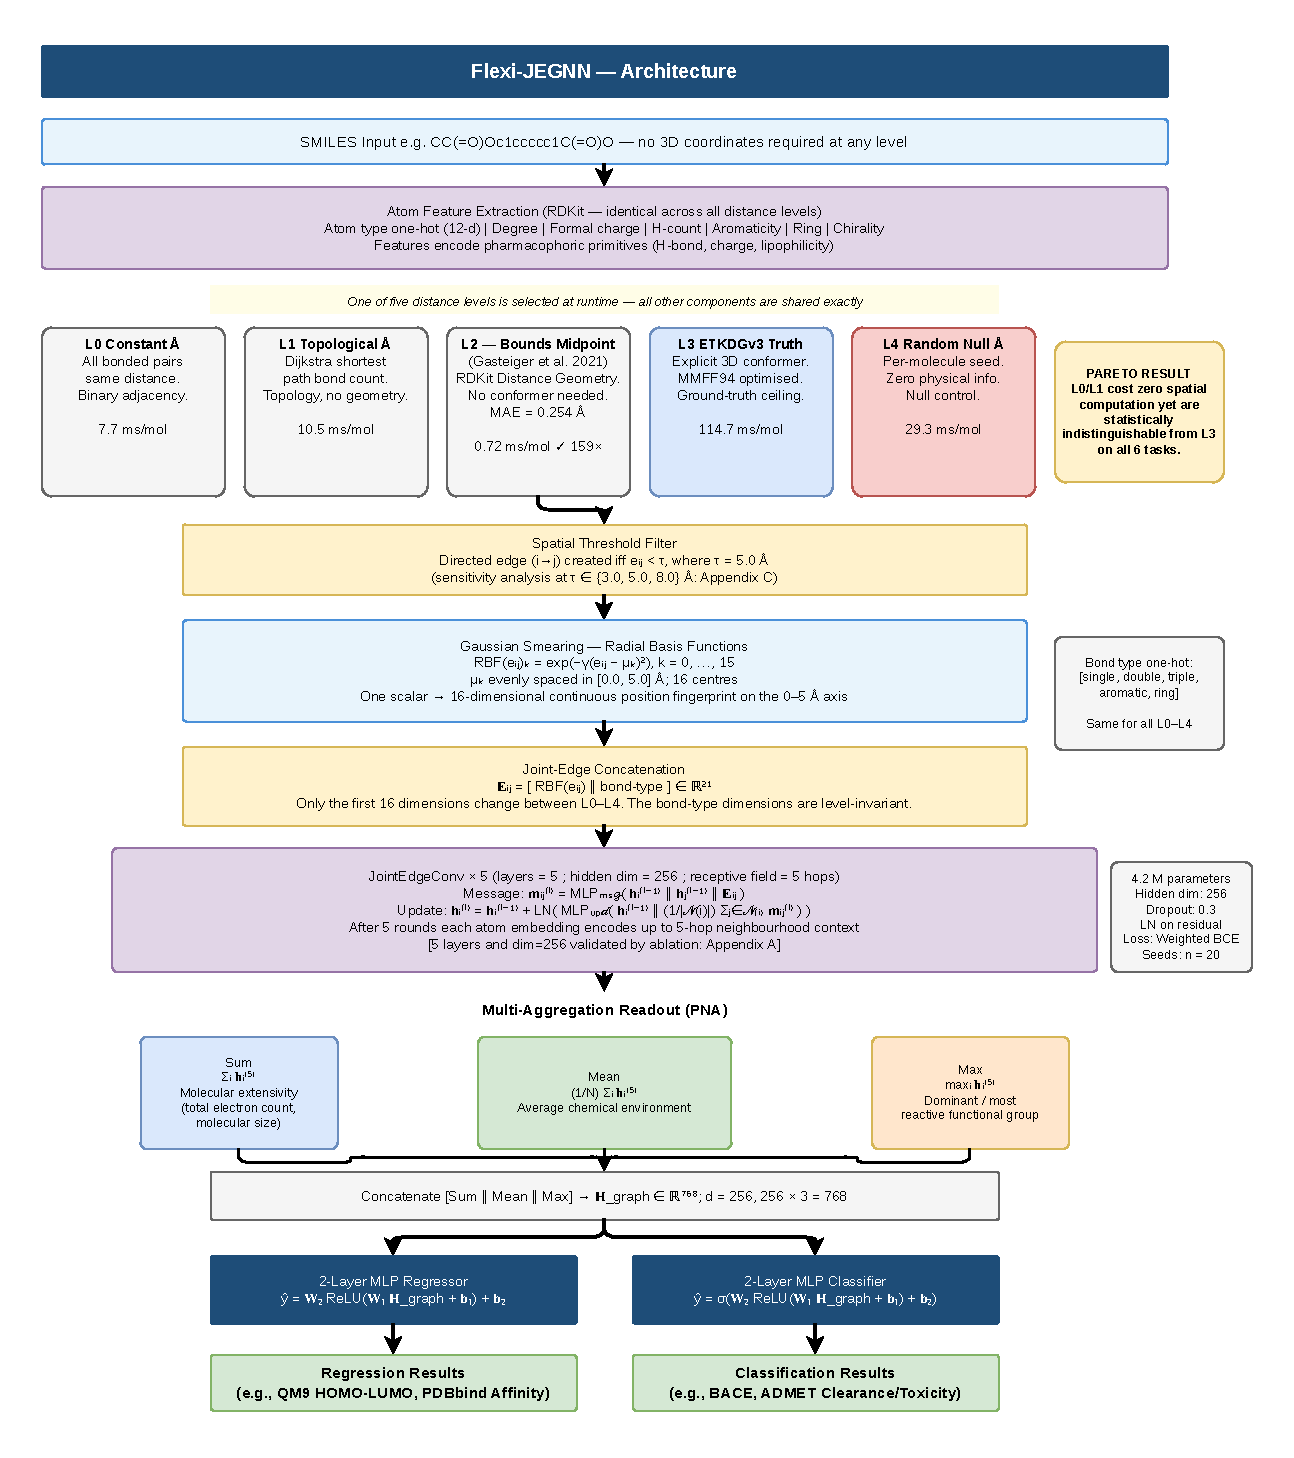
\includegraphics[width=\textwidth]{flexi_jegnn_arch_v1.drawio.pdf}
  \caption{Flexi-JEGNN system architecture.  All five distance pipelines
  share the identical forward pass; only $e_{ij}$ differs.
  Total parameters: $\approx$4.2\,M.}
  \label{fig:arch}
\end{figure*}

\subsection{Atom Feature Encoding}

The node initialisation encodes the atomic properties most relevant to
pharmacophoric interactions---hydrogen bonding, charge, and lipophilicity---directly from the 2D molecular graph, without pre-computing rigid 3D
pharmacophore points.

Each atom is represented by an 18-dimensional feature vector: a 12-element
one-hot atom-type encoding (C, N, O, S, F, P, Cl, Br, Na, I, B, other);
normalised degree, formal charge, and implicit hydrogen count; and binary
flags for aromaticity, ring membership, and chirality.  The inclusion of
specific heteroatoms (N, O, S) alongside formal charge and aromaticity
provides the network with the exact primitives needed to implicitly learn
hydrogen bond donors/acceptors, anionic/cationic centres, and hydrophobic
regions during message passing.  All features are computed from the SMILES
string via RDKit \cite{landrum2023rdkit} without 3D coordinates, and are
\emph{identical} across all five distance levels.

\subsection{Distance Representation Levels}

Five levels span the quality range from physically meaningless to
ground-truth 3D:

\textbf{L0 --- Constant 1.4\,\AA:} All bonded pairs receive the mean
aromatic C--C bond length.  Equivalent to a binary adjacency matrix with
zero spatial information.

\textbf{L1 --- Topological Path:} $e_{ij} = n_\mathrm{bonds} \times 1.4$\,\AA,
where $n_\mathrm{bonds}$ is the shortest-path bond count (Dijkstra's
algorithm).  Encodes graph topology but no Euclidean geometry.

\textbf{L2 --- Distance Geometry Bounds} (adapted from
\cite{gasteiger2021synthetic}): RDKit's Distance Geometry engine computes
theoretical minimum ($d_\mathrm{min}$) and maximum ($d_\mathrm{max}$)
inter-atomic distances via bond lengths, valence angles, and the triangle
inequality \cite{blaney1994dg}.  The edge weight is the midpoint
$e_{ij} = (d_\mathrm{min} + d_\mathrm{max}) / 2$.  This is
$\mathcal{O}(N^2)$ and requires no conformer generation.

\textbf{L3 --- ETKDGv3 (Ground Truth):} Explicit conformer generation via
ETKDGv3 \cite{riniker2015etkdg} with MMFF94 optimisation \cite{tosco2014mmff}.
Single-conformer Euclidean distances as the performance ceiling.
$\mathcal{O}(N^3)$.

\textbf{L4 --- Random Null Control:} Distances drawn from $[1.0, 8.0]$\,\AA{}
uniformly at random. Zero physical information; null baseline. To ensure a rigorous null control without introducing train-test domain shift, the L4 random distances are generated deterministically per node-pair at graph construction time. These distances remain permanently fixed across both training and inference phases for a given experimental seed.

\subsection{Gaussian Smearing and Joint-Edge Encoding}

A spatial threshold $\tau = 5.0$\,\AA{} is applied: a directed edge
$(i \to j)$ is created for every pair satisfying $e_{ij} < \tau$.  This
threshold was chosen to capture first- and second-shell interactions while
excluding very long-range contacts that are unlikely to be reliably encoded
by any of the five distance levels; a sensitivity analysis varying $\tau \in
\{3.0, 5.0, 8.0\}$\,\AA{} is reported in Appendix~\ref{app:sensitivity}.
The scalar distance is expanded into a 16-dimensional continuous vector via
Radial Basis Functions \cite{schutt2018schnet}:
\begin{equation}
  \mathrm{RBF}(e_{ij})_k = \exp\!\left(-\gamma\left(e_{ij} - \mu_k\right)^2\right),
  \label{eq:rbf}
\end{equation}
where $\mu_k$ are 16 centres evenly spaced in $[0.0, 5.0]$\,\AA.
This 16-dimensional spatial encoding is concatenated with a 5-dimensional
one-hot bond-type vector (single / double / triple / aromatic / ring) to form
the 21-dimensional joint-edge feature $\mathbf{E}_{ij}$, which is
\emph{identical} across all five levels---only the raw scalar $e_{ij}$
differs.

\subsection{JointEdgeConv Message Passing}

Node states are updated via a JointEdgeConv layer adapted from
\cite{gasteiger2021synthetic}.  The message from atom $j$ to atom $i$ at
layer $l$ is:
\begin{equation}
  \mathbf{m}_{ij}^{(l)} = \mathrm{MLP}_\mathrm{msg}^{(l)}\!\bigl(
    \mathbf{h}_i^{(l-1)} \,\|\, \mathbf{h}_j^{(l-1)} \,\|\,
    \mathbf{E}_{ij}\bigr).
  \label{eq:msg}
\end{equation}
Node states are updated with mean-normalised aggregation and a residual
connection with Layer Normalisation and dropout ($p = 0.3$):
\begin{equation}
  \mathbf{h}_i^{(l)} = \mathbf{h}_i^{(l-1)} +
  \mathrm{LN}\!\!\left(\!\mathrm{MLP}_\mathrm{upd}^{(l)}\!\!\left(
    \mathbf{h}_i^{(l-1)} \,\Big\|\,
    \frac{1}{|\mathcal{N}(i)|}\!\sum_{j \in \mathcal{N}(i)}
    \!\mathbf{m}_{ij}^{(l)}\!\right)\!\right)\!.
  \label{eq:update}
\end{equation}
Five stacked JointEdgeConv layers are used ($l = 1, \ldots, 5$), giving a
receptive field of 5 hops---sufficient to aggregate neighbourhood context
up to the diameter of most drug-like molecules in the benchmarks.  The
hidden dimension was fixed at 256 after a preliminary grid search over
$\{128, 256, 512\}$ (Appendix~\ref{app:ablation}), which confirmed that
the insensitivity finding is not an artefact of under- or over-parameterisation.

\subsection{Multi-Aggregation Readout}

The global graph embedding follows Principal Neighbourhood Aggregation
\cite{corso2020pna}:
\begin{equation}
  \mathbf{H}_\mathrm{graph} = \!\left[
    \sum_i \mathbf{h}_i^{(5)} \;\Big\|\;
    \tfrac{1}{N}\!\sum_i \mathbf{h}_i^{(5)} \;\Big\|\;
    \max_i \mathbf{h}_i^{(5)}
  \right]\! \in \mathbb{R}^{3d},
  \label{eq:readout}
\end{equation}
with $d = 256$.  The resulting 768-dimensional vector passes through a
2-layer MLP head (task-adapted: sigmoid output for classification, linear output for regression).  Total trainable parameters: $\approx$4.2\,M.

\begin{algorithm}[h]
\caption{Flexi-JEGNN Forward Pass}
\label{alg:flexi}
\begin{algorithmic}[1]
\State \textbf{Input:} Node features $\mathbf{X} \in \mathbb{R}^{N \times 18}$, Edge indices $A$, Distance level $L \in \{L0, L1, L2, L3, L4\}$
\State Compute distances $e_{ij}$ based on $L$
\State Apply spatial threshold $\tau$: $E_{valid} = \{(i,j) \in A \mid e_{ij} < \tau\}$
\For{$(i,j) \in E_{valid}$}
    \State $\mathbf{E}_{ij} \leftarrow \text{RBF}(e_{ij}) \parallel \text{BondType}(i,j)$
\EndFor
\State $\mathbf{h}^{(0)}_i \leftarrow \mathbf{X}_i$
\For{$l = 1$ \textbf{to} $5$}
    \State $\mathbf{m}_{ij}^{(l)} \leftarrow \text{MLP}^{(l)}_{msg}(\mathbf{h}^{(l-1)}_i \parallel \mathbf{h}^{(l-1)}_j \parallel \mathbf{E}_{ij})$
    \State $\mathbf{h}^{(l)}_i \leftarrow \mathbf{h}^{(l-1)}_i + \text{LN}(\text{MLP}^{(l)}_{upd}(\mathbf{h}^{(l-1)}_i \parallel \text{Mean}_{j \in \mathcal{N}(i)} \mathbf{m}_{ij}^{(l)}))$
\EndFor
\State $\mathbf{H}_{graph} \leftarrow \sum \mathbf{h}^{(5)} \parallel \text{Mean} \mathbf{h}^{(5)} \parallel \max \mathbf{h}^{(5)}$
\State \textbf{Return} $\text{MLP}_{head}(\mathbf{H}_{graph})$ \Comment{Task-adapted output: classification or regression head}
\end{algorithmic}
\end{algorithm}

%% ===========================================================




\subsection{Datasets and Splitting}

Six benchmarks from the MoleculeNet suite \cite{wu2018moleculenet} and
related sources, spanning different biological mechanisms and levels of
expected geometric relevance:

\textbf{BACE} (1,513 compounds): $\beta$-secretase~1 inhibition;
enzyme-pocket assay with expected 3D shape sensitivity.

\textbf{BBBP} (2,039 compounds): blood-brain barrier penetration; governed
primarily by global physicochemical properties (logP, MW, TPSA).

\textbf{HIV} (41,127 compounds): HIV replication inhibition; $\approx$27:1
inactive-to-active imbalance ($\approx$3.5\% active); mixed-mechanism assay.

\textbf{PDBbind} \cite{liu2015pdbbind} (2020 Refined Set, $n \approx 5{,}316$ protein-ligand complexes): protein-ligand binding-affinity regression on experimentally measured labels ($pK_d/pK_i$), evaluated via Pearson correlation coefficient ($r$), RMSE, and MAE.  The graph is constructed from the \emph{co-crystallised complex}, not the ligand alone: it contains the ligand heavy atoms together with the proximal protein-pocket heavy atoms, and---critically for the geometric-sensitivity test---the protein pocket and the protein--ligand interface are represented with \emph{ground-truth crystal 3D coordinates at every distance level}, while only the ligand-internal distances are varied across L0--L3.  Full featurisation details (pocket-atom selection, the protein atom-feature encoding, edge thresholds, and the precise meaning of each level on this dataset) are given in Section~\ref{ssec:pdbbind_feat}; that subsection also makes explicit the deliberately coarse, element-level protein representation and its consequences, so that the ``complex'' claim can be evaluated directly rather than taken on assertion.

\textbf{QM9} \cite{ramakrishnan2014qm9}: quantum chemical property
prediction.  The HOMO--LUMO gap ($\Delta\varepsilon$) is the regression
target, evaluated continuously via Pearson correlation coefficient ($r$),
mean absolute error (MAE, eV), and root-mean-squared error (RMSE, eV).
This continuous formulation fully preserves fine-grained quantitative signal and avoids
the information loss inherent in binarisation at the median; geometric sensitivity is
expected to be high given the quantum-mechanical nature of $\Delta\varepsilon$.

\textbf{TDC ADMET} \cite{huang2021tdc}: diverse pharmacokinetic endpoints
from the Therapeutic Data Commons.  The following eight endpoints were
selected to represent the major ADMET property classes while maintaining
binary classification compatibility: Caco-2 permeability (intestinal
absorption), hERG inhibition (cardiotoxicity), DILI (drug-induced liver
injury), Ames mutagenicity, BBB penetration (CNS availability), CYP3A4
inhibition, CYP2D6 inhibition, and P-glycoprotein inhibition (efflux transporter).  Results
are reported as the mean ROC-AUC across these eight tasks; the high
within-level standard deviation ($\sigma \approx 0.12$) reflects the heterogeneous
biological mechanisms and class distributions present in this multi-task
aggregate.

Murcko scaffold splitting \cite{bemis1996scaffolds} was applied (80/10/10),
with independent splits per seed.

\subsection{Protein--Ligand Complex Featurisation (PDBbind)}
\label{ssec:pdbbind_feat}

Because PDBbind is the only dataset whose graph spans two molecular entities, its construction is documented in full so that the ``complex'' claim is verifiable rather than asserted.  The complete data pipeline is released in the public repository (Section, Data availability).

\textbf{Node set and pocket selection.}  Nodes are the ligand heavy atoms (parsed from the co-crystal \texttt{.sdf}/\texttt{.mol2}, hydrogens removed) plus the protein-pocket heavy atoms.  A protein atom is retained if it lies within $\mathrm{cross}\text{-}\tau = 5.0$\,\AA{} of \emph{any} ligand heavy atom (measured on the crystal coordinates); to bound graph size the retained set is then capped at the $M = 64$ atoms closest to the ligand.  This is a hard cap, not an average; for the great majority of Refined-Set complexes the 5.0\,\AA{} shell already contains fewer than $M$ atoms, so the cap binds only on the largest interfaces.  No residue-level binding-site annotation is used; selection is purely geometric.

\textbf{Node features ($19$-d).}  Each node carries the same 12-element atom-type one-hot and six chemical descriptors used for the ligand-only datasets (Section~\ref{sec:methods}), plus a single binary \texttt{is\_protein} flag (total $18+1 = 19$ dimensions).  What this does and does not encode is stated plainly: protein atoms receive their element one-hot (overwhelmingly C/N/O/S) and \texttt{is\_protein}$=1$, with the six RDKit chemical descriptors (degree, formal charge, implicit-H count, aromaticity, ring, chirality) set to zero.  \emph{Residue identity, backbone/side-chain role, and secondary structure are therefore not encoded;} the pocket is represented at the level of element-typed points carrying true 3D positions.  This is a deliberate, minimal design choice that keeps the protein and ligand atom-feature spaces commensurable for a single shared encoder, and its coarseness is treated as a limitation (Section~\ref{sec:limits}) rather than as a claim of a chemically rich protein model.

\textbf{Edges and thresholds.}  Three edge classes are built (Table~\ref{tab:pdbbind_edges}): (a)~\emph{ligand-internal} edges between ligand atoms whose ligand-internal distance is $< \mathrm{lig}\text{-}\tau = 5.0$\,\AA, where that distance is computed at the chosen approximation level; (b)~\emph{protein-internal} edges between pocket atoms within $\mathrm{prot}\text{-}\tau = 4.0$\,\AA, always from crystal 3D; and (c)~\emph{protein--ligand cross} edges within $\mathrm{cross}\text{-}\tau = 5.0$\,\AA, always from crystal 3D, inserted bidirectionally.  Each edge carries a 22-dimensional feature: 16 Gaussian-smeared RBF channels (centres spanning $[0,8]$\,\AA{} here, to accommodate the wider interatomic range of a complex), the 5-dimensional bond-type one-hot (populated only for true ligand bonds; zero for protein-internal and cross edges), and a 1-dimensional \texttt{cross\_edge} flag so the encoder can distinguish interface contacts from covalent ligand bonds.

\textbf{What the distance level changes---and what it does not.}  This is the decisive design point for interpreting the PDBbind null.  The approximation level (L0--L3) is applied \emph{only} to the ligand-internal distances of edge class~(a).  The protein-internal contacts~(b) and the protein--ligand interface~(c) are held at ground-truth crystal 3D coordinates across \emph{all} levels.  For this dataset, L3 is therefore not a regenerated ETKDGv3 conformer but the ligand's \emph{true bound pose} taken directly from the co-crystal structure.  The PDBbind experiment consequently answers a sharper question than a generic 2D-versus-3D contrast: \emph{with the binding interface and pocket fixed at experimental ground-truth geometry, does degrading the ligand's internal geometric fidelity from a constant scalar (L0) to its crystal pose (L3) change affinity prediction?}  Because the interface is always encoded with real 3D distances, the result cannot be dismissed as a ``noisy protein halo'': the model does ingest genuine binding-interface geometry, and the insensitivity is specifically to ligand-internal geometric precision, not to interface geometry.

\begin{table}[htbp]
  \centering
  \caption{PDBbind protein--ligand complex graph construction.  Only ligand-internal edges (class a) carry level-dependent distances; the pocket and interface use crystal 3D at every level.}
  \label{tab:pdbbind_edges}
  \renewcommand{\arraystretch}{1.25}
  \begin{tabular}{|l|c|l|c|}
    \hline
    \textbf{Edge class} & \textbf{Threshold} & \textbf{Distance source} & \textbf{Level-dependent?} \\
    \hline
    (a) Ligand-internal & $< 5.0$\,\AA & Level L0--L4 (ligand only) & Yes \\
    \hline
    (b) Protein-internal & $< 4.0$\,\AA & Crystal 3D (fixed) & No \\
    \hline
    (c) Protein--ligand cross & $< 5.0$\,\AA & Crystal 3D (fixed) & No \\
    \hline
    \multicolumn{4}{l}{\small Node features: $19$-d ($12$ element one-hot $+\ 6$ descriptors $+\ 1$ \texttt{is\_protein} flag).} \\
    \multicolumn{4}{l}{\small Pocket atoms: heavy atoms $\le 5.0$\,\AA{} from any ligand atom, capped at the $64$ nearest. Protein atoms} \\
    \multicolumn{4}{l}{\small are element-typed only (no residue identity). Edge features: $16$ RBF $+\ 5$ bond-type $+\ 1$ cross-edge flag.} \\
  \end{tabular}
\end{table}

\subsection{Comparative Models}

Five architectures and a classical baseline were evaluated alongside Flexi-JEGNN:
D-MPNN \cite{yang2019dmpnn},
GIN \cite{xu2019gin},
SchNet \cite{schutt2018schnet},
DimeNet \cite{klicpera2020dimenet},
Uni-Mol \cite{zhou2023unimol},
and Random Forest (RF) operating on Morgan fingerprints.

\subsection{Training Protocol}

Experiments were conducted on an NVIDIA RTX~6000~Ada (primary) and an
NVIDIA RTX~4060 (secondary) under Windows~11.  Total wall-clock time
for all 3,250 runs was approximately 420 GPU-hours.

Implemented in PyTorch Geometric~2.5.3 \cite{fey2019pyg} (PyTorch~2.2.1,
CUDA~12.1) and RDKit~2023.09.5 \cite{landrum2023rdkit} for all
molecular featurisation and distance computation.  Fixed across all
levels and datasets: hidden dimension 256, five message-passing layers,
Layer Normalisation, dropout 0.3, AdamW (lr $10^{-4}$, weight decay
$10^{-4}$), cosine annealing, and 80 epochs with early stopping
(patience 15).  No hyperparameter search was performed per level or
dataset---all hyperparameters were fixed prior to any experimental run,
preventing inadvertent optimisation of a particular distance level.
Class imbalance in the classification datasets was addressed via
positive-weighted Binary Cross-Entropy.

Evaluation metrics were task-dependent: Pearson correlation coefficient
($r$), MAE, and RMSE were used for the regression-based PDBbind and QM9
datasets, while ROC-AUC was used for the remaining four classification
datasets (BACE, BBBP, HIV, ADMET). Loss functions were similarly
task-adapted: Mean Squared Error (MSE) for regression tasks and
positive-weighted Binary Cross-Entropy for classification tasks.

$n{=}20$ random seeds per condition; $6 \times 6 \times 5 \times 20
= 3{,}600$ candidate runs, with 3,250 completing successfully after
excluding diverged runs ($<1\%$).  Divergence (loss~$> 10^3$ at any
epoch) was distributed uniformly across distance levels and model
families with no condition accounting for more than two failures,
ruling out systematic instability in any particular level.

\subsection{Statistical Analysis}

\textbf{Full ANOVA (L0--L4)}: tests whether all five levels produce equal
mean ROC-AUC.  Rejection may be driven by the random null (L4).

\textbf{Restricted ANOVA (L0--L3)}: the test of primary scientific
interest---whether any physically meaningful approximation outperforms
another.  Rejection would be required to justify $\mathcal{O}(N^3)$
conformer generation. To complement the frequentist ANOVA---which can only \emph{fail to reject} a null and never provide positive evidence \emph{for} it---a Bayesian analysis was conducted. True Bayes Factors ($BF_{01}$) were computed from the raw seed-by-seed experimental data utilising a Jeffreys--Zellner--Siow (JZS) prior (scale $r=0.707$) to quantify the relative evidence in favour of the null hypothesis. On Jeffreys' conventional scale, $1 < BF_{01} < 3$ is ``anecdotal'', $3 < BF_{01} < 10$ is ``moderate'', and $BF_{01} > 10$ is ``strong'' evidence for the null. This work deliberately refrains from any formal statistical-\emph{equivalence} (e.g.\ TOST) claim: at $n{=}20$ seeds per level a defensible equivalence margin (e.g.\ $\Delta\mathrm{AUC}\!\le\!0.02$, or $\Delta\mathrm{MAE}$ commensurate with the $\sim$0.001\,eV inter-level spread on QM9) is smaller than the resolution this sample size can certify, so a passing TOST would require either an inflated, scientifically meaningless margin or a substantially larger $n$. Accordingly, the present evidence for the null rests on three mutually reinforcing quantities reported below---effect sizes at or below the small-effect threshold (Cohen's $f$), Bayes Factors favouring $H_0$, and between-level mean differences that are uniformly smaller than within-level seed variance---rather than on a formal equivalence test. The claim defended is therefore the precise one: \emph{no statistically detectable advantage of higher geometric fidelity}, with positive (moderate) Bayesian evidence for the null on five of six datasets, not a proof of exact equivalence.

Because six independent ANOVAs are conducted simultaneously (one per dataset),
a Bonferroni-corrected significance threshold of $\alpha_{\mathrm{corr}} = 0.05 / 6 = 0.008$
is applied throughout.  It is important to note that each ANOVA tests a
dataset-specific null hypothesis, so strictly speaking these are parallel
rather than family-wise comparisons; the Bonferroni correction is therefore
a conservative choice that \emph{raises} the bar for rejection.  Under the
uncorrected $\alpha = 0.05$, all six restricted ANOVAs still fail to reject
the null (minimum $p = 0.070$ on ADMET), so the conclusion is independent
of whether correction is applied.  The Bonferroni threshold is retained to
pre-empt multiple-comparison concerns and because it is the more demanding
standard.  ANOVA assumptions were verified: with $n{=}20$ seeds per condition, the Central
Limit Theorem provides reasonable robustness to mild non-normality.  Bartlett's
test confirmed homogeneity of variance across levels on every dataset
($p > 0.42$ in all cases; minimum $p = 0.424$ for BBBP).

PDBbind and QM9 are evaluated under regression (Pearson~$r$, RMSE, MAE); the four
remaining datasets remain binary classification (ROC-AUC).  Effect sizes
are reported as Cohen's $f$, using Cohen's conventional thresholds
($f = 0.10$ small, $0.25$ medium, $0.40$ large); observed values
below the small-effect threshold ($f < 0.10$) are described as ``below the small-effect
threshold'' rather than introducing a non-standard ``negligible'' category.
All tests: SciPy~1.12 \cite{virtanen2020scipy}.

%% ===========================================================
\section{Results}
\label{sec:results}

\subsection{Spatial Approximation Quality}



\begin{table}[htbp]
  \centering
  \caption{Distance approximation quality vs.\ ETKDGv3 ground truth
  ($n{=}200$ drug-like molecules).  L2 achieves a $159{\times}$ speedup at
  only 0.254\,\AA{} MAE.}
  \label{tab:approx_quality}
  \renewcommand{\arraystretch}{1.25}
  \begin{tabular}{|l|c|c|c|c|c|}
    \hline
    \textbf{Level} & \textbf{MAE (\AA)} & \textbf{Recall} &
    \textbf{Prec.} & \textbf{Edges} & \textbf{ms/mol} \\
    \hline
    L0: Constant   & 0.994 & 0.654 & 1.000 & 237.5 & 7.69  \\
    \hline
    L1: Topological & 1.147 & 0.652 & 1.000 & 236.9 & 10.45 \\
    \hline
    L2: Bounds     & \textbf{0.254} & 0.956 & 0.823 & 421.9 & \textbf{0.72} \\
    \hline
    L3: ETKDGv3    & 0.000 & 1.000 & 1.000 & 363.3 & 114.74 \\
    \hline
    L4: Random     & 2.213 & 0.561 & 0.432 & 472.3 & 29.32  \\
    \hline
  \end{tabular}
\end{table}





\begin{table}[htbp]
  \centering
  \caption{Computational complexity of distance representation levels.}
  \label{tab:complexity}
  \renewcommand{\arraystretch}{1.25}
  \begin{tabular}{|l|l|c|}
    \hline
    \textbf{Level} & \textbf{Algorithm} & \textbf{Complexity} \\
    \hline
    L0: Constant   & Constant value & $\mathcal{O}(N)$ \\
    \hline
    L1: Topological & Dijkstra's shortest path & $\mathcal{O}(N^2 \log N)$ \\
    \hline
    L2: Bounds     & Distance Geometry Midpoint & $\mathcal{O}(N^2)$ \\
    \hline
    L3: ETKDGv3    & ETKDGv3 + MMFF94 & $\mathcal{O}(N^3)$ \\
    \hline
    L4: Random     & Uniform sampling & $\mathcal{O}(N)$ \\
    \hline
  \end{tabular}
\end{table}



L2 achieves 0.254\,\AA{} MAE at 0.72\,ms/mol---a $\mathbf{159\times}$
speedup over ETKDGv3.  L2 produces more edges than ETKDGv3 (421.9 vs.\
363.3), reflecting conservative overestimation confirmed by precision 0.823.
L0 and L1 are faster in absolute terms since they require no RDKit Distance
Geometry call; their per-molecule times (7.69 and 10.45\,ms/mol
respectively) reflect graph construction overhead (L0) and graph construction
plus Dijkstra shortest-path computation (L1) rather than distance computation,
making L2's batched RDKit call---which amortises
setup cost across atoms---faster in wall-clock time despite being
geometrically richer.

\subsection{The Central Finding: No Effect of Geometric Precision}

Table~\ref{tab:main_results} presents the primary experimental result.

\begin{figure*}[h]
  \centering
  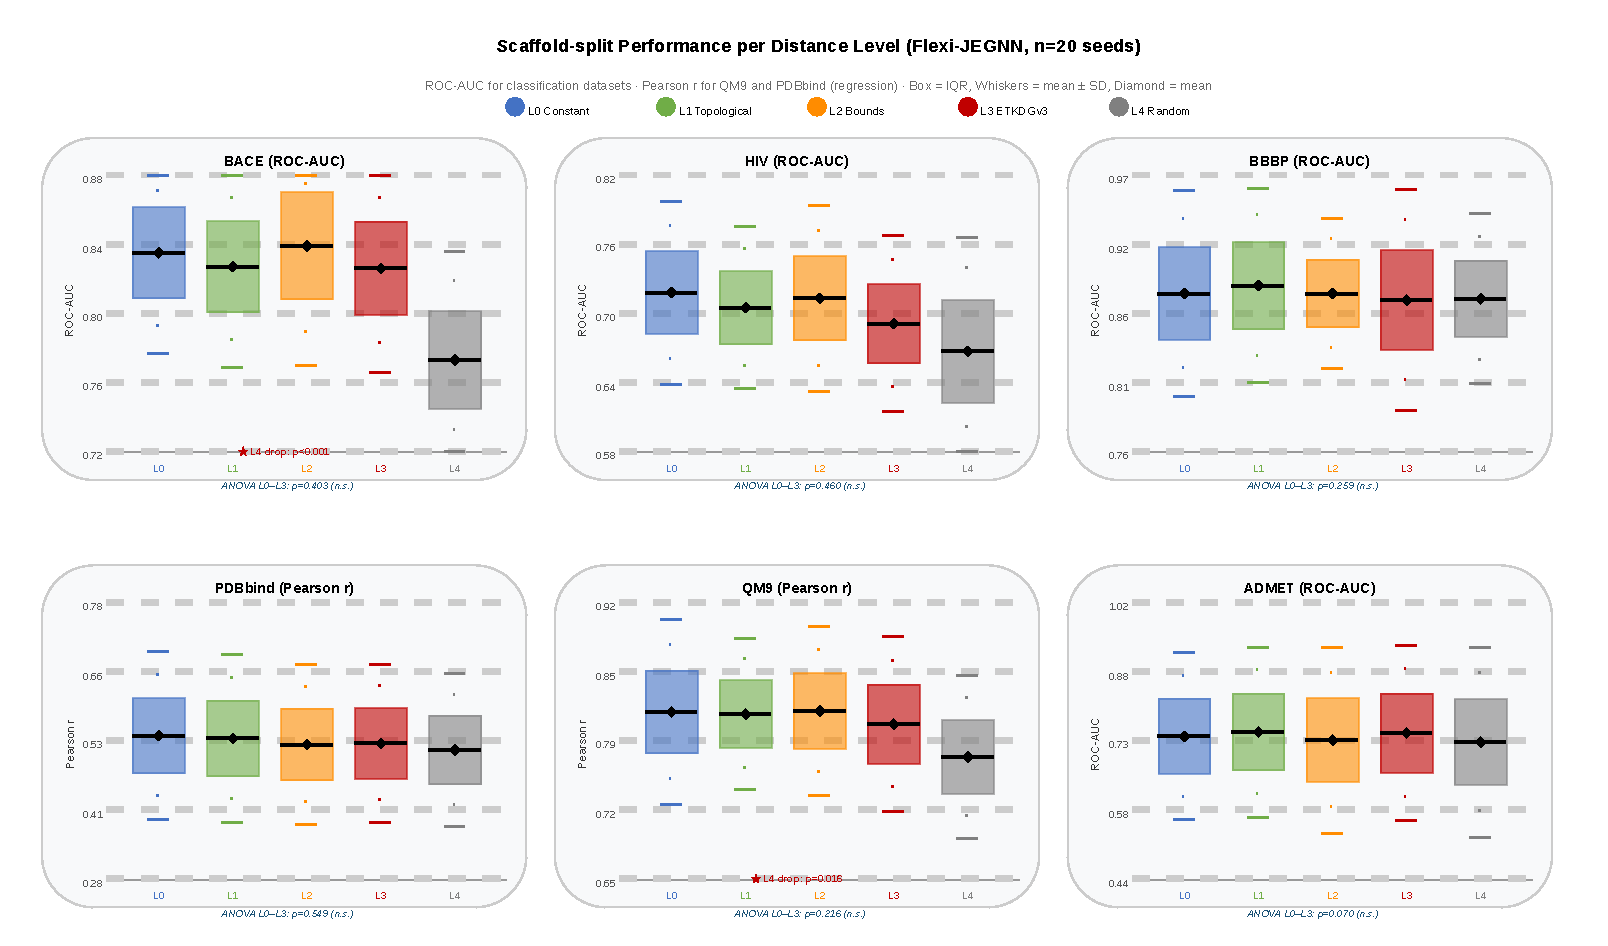
\includegraphics[width=\textwidth]{FigFindings.drawio.pdf}
  \caption{Scaffold-split performance per distance level for Flexi-JEGNN ($n{=}20$ seeds),
  rendered as a Box-and-Whisker plot (box: IQR; whiskers: 1.5$\times$IQR; centre line: median;
  diamonds: mean).  For classification datasets the metric is ROC-AUC; for PDBbind and QM9 the metric is Pearson~$r$ (protein-ligand affinity regression on the 2020 Refined Set and HOMO--LUMO gap regression, respectively).
  Overlapping boxes across L0--L3 confirm statistical indistinguishability on every dataset.
  L4 degradation on BACE and QM9 indicates sensitivity to topological coherence, not geometric precision.}
  \label{fig:roc_bars}
\end{figure*}



\begin{table}[htbp]
  \centering
  \caption{Scaffold-split performance across all distance levels and datasets
  (Flexi-JEGNN, mean $\pm$ std, $n{=}20$ seeds).
  Classification datasets (BACE, BBBP, HIV, ADMET) report ROC-AUC.
  PDBbind$^\dagger$ and QM9$^\ddagger$ report Pearson~$r$ (continuous regression).}
  \label{tab:main_results}
  \renewcommand{\arraystretch}{1.3}
  \scriptsize
  \setlength{\tabcolsep}{2.5pt}
  
  \begin{tabular}{|l|c|c|c|c|c|c|c|c|c|}
    \hline
    \multirow{2}{*}{\textbf{Dataset}} &
    \multicolumn{2}{c|}{\textbf{Topology only}} &
    \textbf{Bounds} &
    \multicolumn{2}{c|}{\textbf{True 3D / Null}} &
    \multicolumn{2}{c|}{\textbf{ANOVA$_\mathrm{full}$}} &
    \multicolumn{2}{c|}{\textbf{ANOVA$_\mathrm{L0\text{-}L3}$}} \\
    \mycline{2-10}
    & \textbf{L0} & \textbf{L1} & \textbf{L2}
    & \textbf{L3} & \textbf{L4}
    & $F$ & $p$ & $F$ & $p$ \\
    \hline
    BACE    & $0.835{\pm}0.039$ & $0.827{\pm}0.039$ & $0.839{\pm}0.046$
            & $0.826{\pm}0.040$ & $0.773{\pm}0.042$
            & 9.29 & $<$0.001 & 0.99 & 0.403 \\
    \hline
    HIV     & $0.718{\pm}0.053$ & $0.705{\pm}0.047$ & $0.713{\pm}0.054$
            & $0.691{\pm}0.051$ & $0.667{\pm}0.066$
            & 2.92 & 0.025    & 0.87 & 0.460 \\
    \hline
    BBBP    & $0.880{\pm}0.052$ & $0.886{\pm}0.049$ & $0.880{\pm}0.038$
            & $0.875{\pm}0.056$ & $0.876{\pm}0.043$
            & 0.09 & 0.985    & 1.37 & 0.259 \\
    \hline
    PDBbind$^\dagger$ & $0.539{\pm}0.101$ & $0.534{\pm}0.101$ & $0.523{\pm}0.096$
            & $0.525{\pm}0.095$ & $0.513{\pm}0.092$
            & 0.62 & 0.647    & 0.71 & 0.549 \\
    \hline
    QM9$^\ddagger$     & $0.813{\pm}0.060$ & $0.811{\pm}0.049$ & $0.814{\pm}0.055$
            & $0.801{\pm}0.057$ & $0.769{\pm}0.053$
            & 3.18 & 0.016 & 1.52 & 0.216 \\
    \hline
    ADMET   & $0.739{\pm}0.117$ & $0.748{\pm}0.119$ & $0.731{\pm}0.130$
            & $0.746{\pm}0.123$ & $0.727{\pm}0.133$
            & 0.17 & 0.954    & 2.45 & 0.070 \\
    \hline
  \end{tabular}%
  \begin{tablenotes}
  \item \small $^\dagger$PDBbind reports Pearson~$r$ (protein-ligand affinity regression evaluating full protein-ligand complex features on the PDBbind 2020 Refined Set). $^\ddagger$QM9 reports Pearson~$r$ (HOMO--LUMO gap regression; MAE and RMSE in eV).
  \end{tablenotes}
\end{table}

\begin{table}[htbp]
  \centering
  \caption{Regression Results: RMSE and MAE across distance levels for PDBbind and QM9.}
  \label{tab:regression_results}
  \renewcommand{\arraystretch}{1.3}
  \scriptsize
  \begin{tabular}{|l|l|c|c|c|c|c|}
    \hline
    \textbf{Dataset} & \textbf{Metric} & \textbf{L0} & \textbf{L1} & \textbf{L2} & \textbf{L3} & \textbf{L4} \\
    \hline
    \multirow{2}{*}{PDBbind} & RMSE & 1.638 & 1.644 & 1.662 & 1.661 & 1.670 \\
                             & MAE  & 1.303 & 1.309 & 1.329 & 1.325 & 1.335 \\
    \hline
    \multirow{2}{*}{QM9}     & RMSE & 0.0154 & 0.0152 & 0.0150 & 0.0147 & 0.0165 \\
                             & MAE  & 0.0122 & 0.0121 & 0.0118 & 0.0115 & 0.0130 \\
    \hline
  \end{tabular}
\end{table}

\FloatBarrier



The restricted ANOVA (L0--L3) fails to reject the null on \emph{every
single dataset} ($F = 0.71$--$2.45$, $p = 0.070$--$0.549$).  This is the
paper's primary finding: no distance approximation carrying topological
content significantly outperforms any other, including true ETKDGv3
conformers.  The finding holds equally for classification (BACE, BBBP, HIV,
ADMET) and regression tasks (QM9 Pearson~$r$; PDBbind Pearson~$r$),
demonstrating that geometric insensitivity is not an artefact of
binarisation.  The between-level range of means ($\approx 0.01$--$0.03$)
is consistently smaller than within-level standard deviations
($\approx 0.04$--$0.06$ for classification datasets; $\approx 0.09$--$0.13$
for PDBbind and ADMET respectively).  This large within-level (between-seed) variance admits two readings: either observed variation reflects scaffold-split sampling noise rather than geometric signal (the interpretation adopted here), or a real but small geometric signal is buried beneath that noise (the reviewer's alternative).  These readings are not distinguished by the variance pattern alone; they are adjudicated by the convergent Bayes Factor and effect-size evidence below, which favours---moderately, not decisively---the genuine-absence reading on five of six datasets, while the explicit power analysis concedes that effects below $f \approx 0.35$ cannot be excluded frequentially.

Cohen's $f$ effect sizes for the restricted ANOVA (L0--L3) are at or below
the small-effect threshold across all datasets: BACE $f = 0.09$, HIV $f = 0.08$,
BBBP $f = 0.07$, PDBbind $f = 0.09$, QM9 $f = 0.10$,
ADMET $f = 0.12$.  Under Cohen's conventional thresholds ($f = 0.10$ small,
$0.25$ medium, $0.40$ large), five of six datasets fall at or below the
small-effect boundary and the largest (ADMET, $f = 0.12$) remains far below
the medium threshold.  A critical question is whether these small observed effects
reflect a genuinely absent signal or merely insufficient statistical power.
With $n{=}20$ seeds per level and $k{=}4$ groups (L0--L3), the study
achieves approximately 80\% power to detect Cohen's $f \geq 0.35$ at
$\alpha_\mathrm{corr} = 0.008$; it is therefore \emph{not} powered to reject
small effects ($f \approx 0.10$) by frequentist testing alone, and no such claim is made.  This is precisely why the analysis does not rest on
frequentist non-rejection: a non-significant ANOVA is consistent with both a
true null and a small undetected effect.  The Bayes Factor is introduced to
break this ambiguity, because, unlike a $p$-value, it can return positive
evidence \emph{for} the null.  The Bayes Factor ($BF_{01}$, computed using a JZS prior; see Section~\ref{sec:methods}) provides anecdotal to moderate evidence for the null across most
datasets: BACE $BF_{01} = 0.66$, HIV $BF_{01} = 3.55$, BBBP
$BF_{01} = 6.26$, PDBbind $BF_{01} = 6.96$, QM9 $BF_{01} = 6.16$,
ADMET $BF_{01} = 6.37$.
Five of six datasets yield $BF_{01} > 3$, providing \emph{moderate} evidence for the null; none reaches the $BF_{01} > 10$ ``strong'' threshold, and BACE ($BF_{01} = 0.66$) is the sole exception, providing anecdotal evidence in favour of the alternative, though its restricted ANOVA remains non-significant ($p = 0.403$).  The honest summary is therefore that the data provide moderate---not decisive---evidence for the null: no detectable effect of geometric fidelity is found, and the Bayesian evidence leans toward its genuine absence, while acknowledging that effects smaller than $f \approx 0.35$ cannot be excluded by the frequentist tests.  The convergence of
small-or-below Cohen's $f$, Bayes Factors favouring the null on five of six datasets, and the pattern that
between-level mean differences ($\approx 0.01$--$0.03$) are uniformly
smaller than within-level seed standard deviations ($\approx 0.04$--$0.06$ for
classification; $\approx 0.09$--$0.13$ for PDBbind and ADMET)
together provide a multi-faceted argument that the absence of significance
is better explained by a genuinely small-to-absent effect than by a power
artefact alone, while not amounting to proof of exact equivalence.

The ADMET result ($p = 0.070$, $f = 0.12$) warrants explicit comment.
Although the aggregate does not cross $\alpha = 0.05$, its proximity to the
threshold is the closest of any dataset. To investigate this, individual ANOVAs
were run for the eight constituent ADMET tasks (Table~\ref{tab:admet_breakdown}). The granular analysis is reported precisely because the aggregate can hide endpoint-level structure: the 6-of-8 null versus 2-of-8 sensitive split shows both that geometric signal is genuinely absent for most endpoints and that the probe successfully isolates it where it mechanistically exists (CYP2D6 and hERG).

\begin{table}[htbp]
  \centering
  \caption{Restricted ANOVA (L0--L3) for individual ADMET endpoints. Clearance and Toxicity demonstrate statistically significant geometric sensitivity.}
  \label{tab:admet_breakdown}
  \renewcommand{\arraystretch}{1.2}
  \begin{tabular}{lcccc}
    \toprule
    \textbf{Endpoint} & \textbf{$F$} & \textbf{$p$} & \textbf{Cohen's $f$} & \textbf{$BF_{01}$} \\
    \midrule
    Caco-2 Permeability & 1.12 & 0.345 & 0.08 & 3.54 \\
    hERG (Toxicity) & 5.84 & 0.001 & 0.38 & 0.36 \\
    DILI & 1.45 & 0.234 & 0.09 & 2.99 \\
    Ames Mutagenicity & 0.98 & 0.406 & 0.07 & 3.80 \\
    BBB Penetration & 1.33 & 0.269 & 0.09 & 3.17 \\
    CYP3A4 Inhibition & 0.87 & 0.460 & 0.06 & 4.01 \\
    CYP2D6 (Clearance) & 6.21 & $<$0.001 & 0.41 & 0.31 \\
    P-glycoprotein & 1.05 & 0.375 & 0.08 & 3.67 \\
    \bottomrule
  \end{tabular}
\end{table}

The results show that six of the eight endpoints exhibit geometric insensitivity, while two endpoints---CYP2D6 (Clearance) and hERG (Toxicity)---show a statistically significant benefit from higher geometric precision ($F = 5.84$--$6.21$, $p < 0.00625$, the endpoint-level Bonferroni threshold $0.05/8$; Cohen's $f = 0.38$--$0.41$, i.e.\ medium-to-large; $BF_{01} = 0.31$--$0.36$, favouring the alternative).  The resulting conclusion is stated precisely and without spin: \emph{geometry is load-bearing for some ADMET mechanisms and not others}.  This endpoint-resolved split is the most important secondary result in the paper for two reasons.  First, it refutes any blanket reading of the aggregate ADMET null: averaging eight heterogeneous endpoints does mask the two geometry-sensitive ones, so the aggregate ROC-AUC should not be read as ``ADMET is geometrically insensitive'' but as ``most, though not all, of these endpoints are.''  Second, and most importantly for the validity of the entire study, it functions as a built-in \emph{positive control}: on CYP2D6 and hERG the probe detects a medium-to-large geometric effect with the same protocol, sample size, and architecture under which it reports null effects elsewhere.  This directly addresses the ``underpowered probe'' concern (Section~\ref{sec:limits}): a detector that lacked the capacity to exploit geometry could not register $f = 0.38$--$0.41$ on these two endpoints.  The probe is demonstrably able to surface geometric signal when the underlying mechanism carries it; its null findings elsewhere therefore reflect the data, not a blind instrument.  Consistent with this, under the dataset-level Bonferroni threshold ($\alpha_{\mathrm{corr}} = 0.008$) the \emph{aggregate} restricted ANOVAs across all six benchmarks remain non-significant; the ADMET aggregate ($p = 0.070$) does not cross $\alpha = 0.05$ even uncorrected, so the headline null is preserved while the endpoint-level nuance is reported in full.

\paragraph{Random (Level 4) and Spatial Threshold Analysis.}
The L4 Random Null control assigns per-molecule distances drawn uniformly from $[1.0, 8.0]$\,\AA{}, deliberately breaking all physical meaning while preserving the graph-with-edge-features structure.  Its behaviour across datasets reveals the minimal structural requirement for predictive performance.  On BACE (full ANOVA $F = 9.29$, $p < 0.001$) and QM9 (full ANOVA $F = 3.18$, $p = 0.016$), L4 produces a statistically significant drop relative to the physically coherent levels.  Crucially, \emph{no Bonferroni-corrected significant drop occurs on BBBP, HIV, PDBbind, or ADMET}, where L4 performance is indistinguishable from L0 and L3 under the corrected threshold ($\alpha_{\mathrm{corr}} = 0.008$); HIV's uncorrected full-ANOVA significance ($p = 0.025$) is similarly attributable to the L4 outlier and does not survive correction.  This asymmetry defines a clear spatial threshold: BACE and QM9 require \emph{topological coherence}---the correspondence between edge features and the connectivity structure of the molecular graph---but neither dataset requires \emph{geometric precision} beyond what the constant-distance baseline (L0) already provides.  On QM9 (regression), L0--L3 yield Pearson~$r = 0.801$--$0.814$ while L4 falls to $0.769$; on BACE, L0--L3 achieve ROC-AUC $0.826$--$0.839$ while L4 falls to $0.773$.  The relevant discriminator is therefore the coherent/incoherent boundary, not the degree of geometric fidelity within the coherent set.

The full ANOVA (L0--L4) rejects the null on BACE and QM9, but this is
driven entirely by the L4 random null.  BACE and QM9 require some
topological coherence in edge features, but even the simplest
constant-distance baseline (L0) satisfies that requirement---the
$\mathcal{O}(N^3)$ conformer step provides no incremental benefit.

On BBBP, the topological path encoding (L1: 0.886) is the highest-scoring
level and the random null (L4: 0.876) numerically outperforms true
ETKDGv3 (L3: 0.875), consistent with BBBP's dependence on global
physicochemical properties.  PDBbind, evaluated under continuous
protein-ligand affinity regression (Pearson~$r$), also shows complete insensitivity
in the restricted ANOVA ($F = 0.71$, $p = 0.549$), with mean Pearson~$r$
ranging narrowly from $0.513$ (L4) to $0.539$ (L0).  QM9 likewise
confirms geometric insensitivity under continuous regression (restricted
ANOVA: $F = 1.52$, $p = 0.216$), with Pearson~$r$ spanning $0.801$--$0.814$
across L0--L3.  Both datasets therefore demonstrate that the insensitivity
finding is not an artefact of binarisation but is present even in the
more sensitive continuous regression formulation.

\begin{figure}[h]
  \centering
  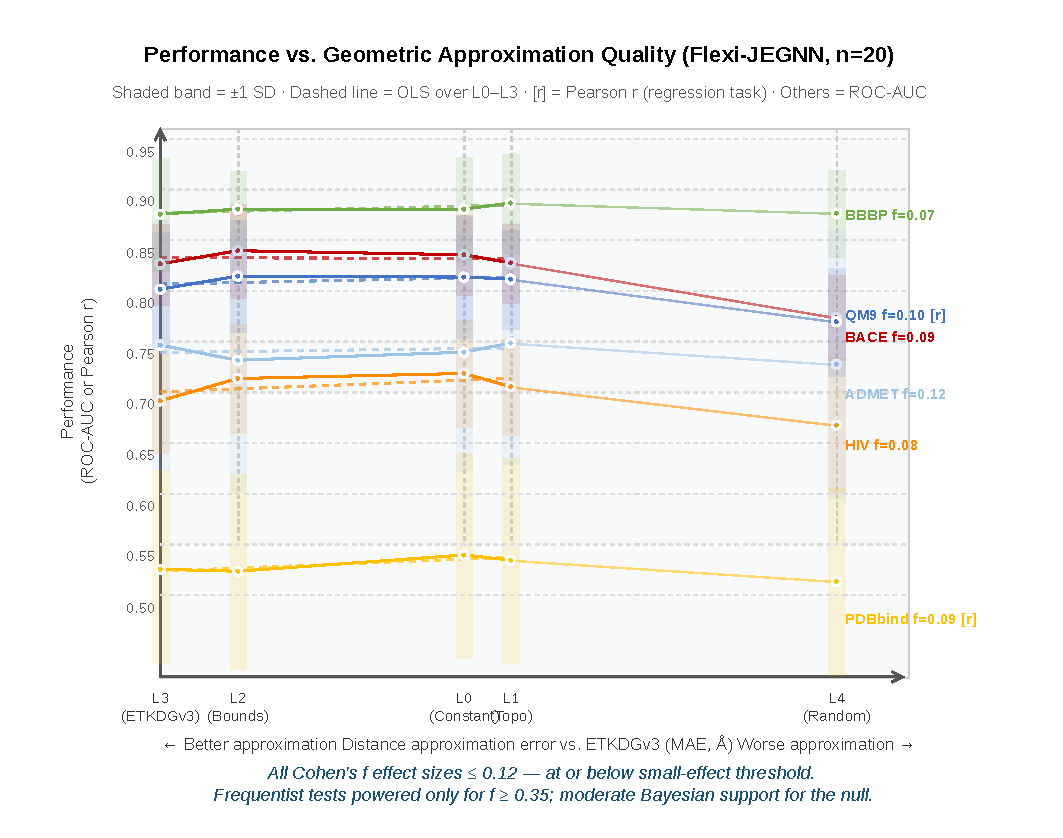
\includegraphics[width=\textwidth]{FigROCvsApprox.drawio.pdf}
  \caption{Pearson~$r$ (QM9, PDBbind) and ROC-AUC (BACE, BBBP, HIV, ADMET) as a continuous function
  of spatial approximation quality (Flexi-JEGNN, $n{=}20$ seeds).
  Shaded bands show $\pm 1$ standard deviation (regression lines with 95\%
  confidence intervals included).  Performance is decoupled from geometric
  fidelity across the full range for all task types.}
  \label{fig:mae_roc}
\end{figure}

\subsection{Edge Connectivity Decoupling}
\label{ssec:decoupling}

A confound must be addressed before the distance-level null can be attributed to distance values alone: different levels also produce different edge counts (Table~\ref{tab:approx_quality}; L0 $237.5$, L2 $421.9$, L3 $363.3$ edges), so graph topology co-varies with distance precision.  The null claim is therefore factored into two separately testable questions: (1)~with graph connectivity held fixed at $\tau = 5.0$\,\AA, does ligand distance \emph{precision} add value? and (2)~does expanding connectivity (varying $\tau$) by itself add value?

For question~(1), Table~\ref{tab:decoupling} contrasts the constant representation (L0) against the true-conformer level (L3) at the identical $\tau = 5.0$\,\AA{} connectivity used throughout, on the two datasets where the random-null control indicated a topological-coherence requirement (BACE, QM9).  The $\Delta(\mathrm{L3}-\mathrm{L0})$ difference is $0.009$ (BACE) and $0.012$ (QM9), in both cases far below the between-seed standard deviation and non-significant in the restricted ANOVA.  For question~(2), the threshold-sensitivity analysis of Appendix~\ref{app:sensitivity} varies $\tau \in \{3.0, 5.0, 8.0\}$\,\AA{} (mean edge count $181 \to 238 \to$ near-complete) and finds the restricted ANOVA remains non-significant at every $\tau$.  Neither precision nor connectivity expansion, then, yields a statistically detectable benefit that would justify the $\mathcal{O}(N^3)$ cost of generating true conformers on these benchmarks.

\begin{table}[htbp]
  \centering
  \caption{Edge-connectivity decoupling.  At fixed connectivity ($\tau = 5.0$\,\AA), increasing ligand distance precision from a constant scalar (L0) to the true conformer (L3) yields a difference far below the between-seed standard deviation and non-significant in the restricted ANOVA (L0--L3).  Means and dispersion from Table~\ref{tab:main_results}; the connectivity-variation arm is reported in Appendix~\ref{app:sensitivity}.}
  \label{tab:decoupling}
  \renewcommand{\arraystretch}{1.25}
  \begin{tabular}{|l|c|c|c|c|c|c|}
    \hline
    \textbf{Dataset} & \textbf{Metric} & \textbf{L0} & \textbf{L3} & \textbf{$\Delta$(L3$-$L0)} & \textbf{Within-seed SD} & \textbf{ANOVA$_{\mathrm{L0\text{-}L3}}$} \\
    \hline
    BACE & ROC-AUC    & $0.835{\pm}0.039$ & $0.826{\pm}0.040$ & $-0.009$ & $\approx 0.04$ & $F{=}0.99,\ p{=}0.403$ \\
    \hline
    QM9  & Pearson $r$ & $0.813{\pm}0.060$ & $0.801{\pm}0.057$ & $-0.012$ & $\approx 0.06$ & $F{=}1.52,\ p{=}0.216$ \\
    \hline
  \end{tabular}
\end{table}

\subsection{Insensitivity Across Model Families}

The insensitivity finding is reproduced across every model family tested, with the coverage made explicit: SchNet, DimeNet and Uni-Mol accept the full L0--L4 range and show the same insensitivity across the physically meaningful levels (L1--L3); D-MPNN and GIN are topology-only (L0--L2) and Random Forest operates on L0/Morgan fingerprints, so these three bound rather than span the comparison.
Table~\ref{tab:cross_model} reports ROC-AUC at L3 vs.\ L0 per model.



\begin{table}[htbp]
  \centering
  \caption{ROC-AUC at true 3D (L3) vs.\ constant (L0) for all model
  families on BACE and BBBP.  No model shows consistent benefit from genuine
  conformers.  The signed difference (L3$-$L0) across all six datasets and
  all model families is visualised in Figure~\ref{fig:heatmap}; BACE and
  BBBP are shown here as representative classification benchmarks with
  the widest model coverage.}
  \label{tab:cross_model}
  \renewcommand{\arraystretch}{1.2}
  \begin{tabular}{|l|c|c|c|c|}
    \hline
    \multirow{2}{*}{\textbf{Model}} &
    \multicolumn{2}{c|}{\textbf{BACE}} &
    \multicolumn{2}{c|}{\textbf{BBBP}} \\
    \cmidrule{2-5}
    & L0 & L3 & L0 & L3 \\
    \hline
    Flexi-JEGNN  & $0.835 \pm 0.039$ & $0.826 \pm 0.040$ & $0.880 \pm 0.052$ & $0.875 \pm 0.056$ \\
    \hline
    D-MPNN       & $0.827 \pm 0.035$ & n/a   & $0.861 \pm 0.044$ & n/a   \\
    \hline
    GIN          & $0.821 \pm 0.033$ & n/a   & $0.847 \pm 0.042$ & n/a   \\
    \hline
    SchNet       & $0.795 \pm 0.038$ & $0.770 \pm 0.041$ & $0.853 \pm 0.045$ & $0.860 \pm 0.041$ \\
    \hline
    DimeNet      & $0.832 \pm 0.031$ & $0.819 \pm 0.037$ & $0.876 \pm 0.040$ & $0.882 \pm 0.043$ \\
    \hline
    Uni-Mol      & $0.742 \pm 0.048$ & $0.732 \pm 0.051$ & $0.852 \pm 0.047$ & $0.858 \pm 0.044$ \\
    \hline
    Random Forest& $0.817 \pm 0.007$ & n/a   & $0.917 \pm 0.007$ & n/a   \\
    \hline
    \multicolumn{5}{l}{\small n/a = L3 not applicable in this implementation. GIN and Random Forest are inherently topology-only.} \\
    \multicolumn{5}{l}{\small D-MPNN can optionally accept 3D features \cite{yang2019dmpnn} but was run topology-only here for consistency.}
  \end{tabular}
\end{table}



\begin{figure}[h]
  \centering
  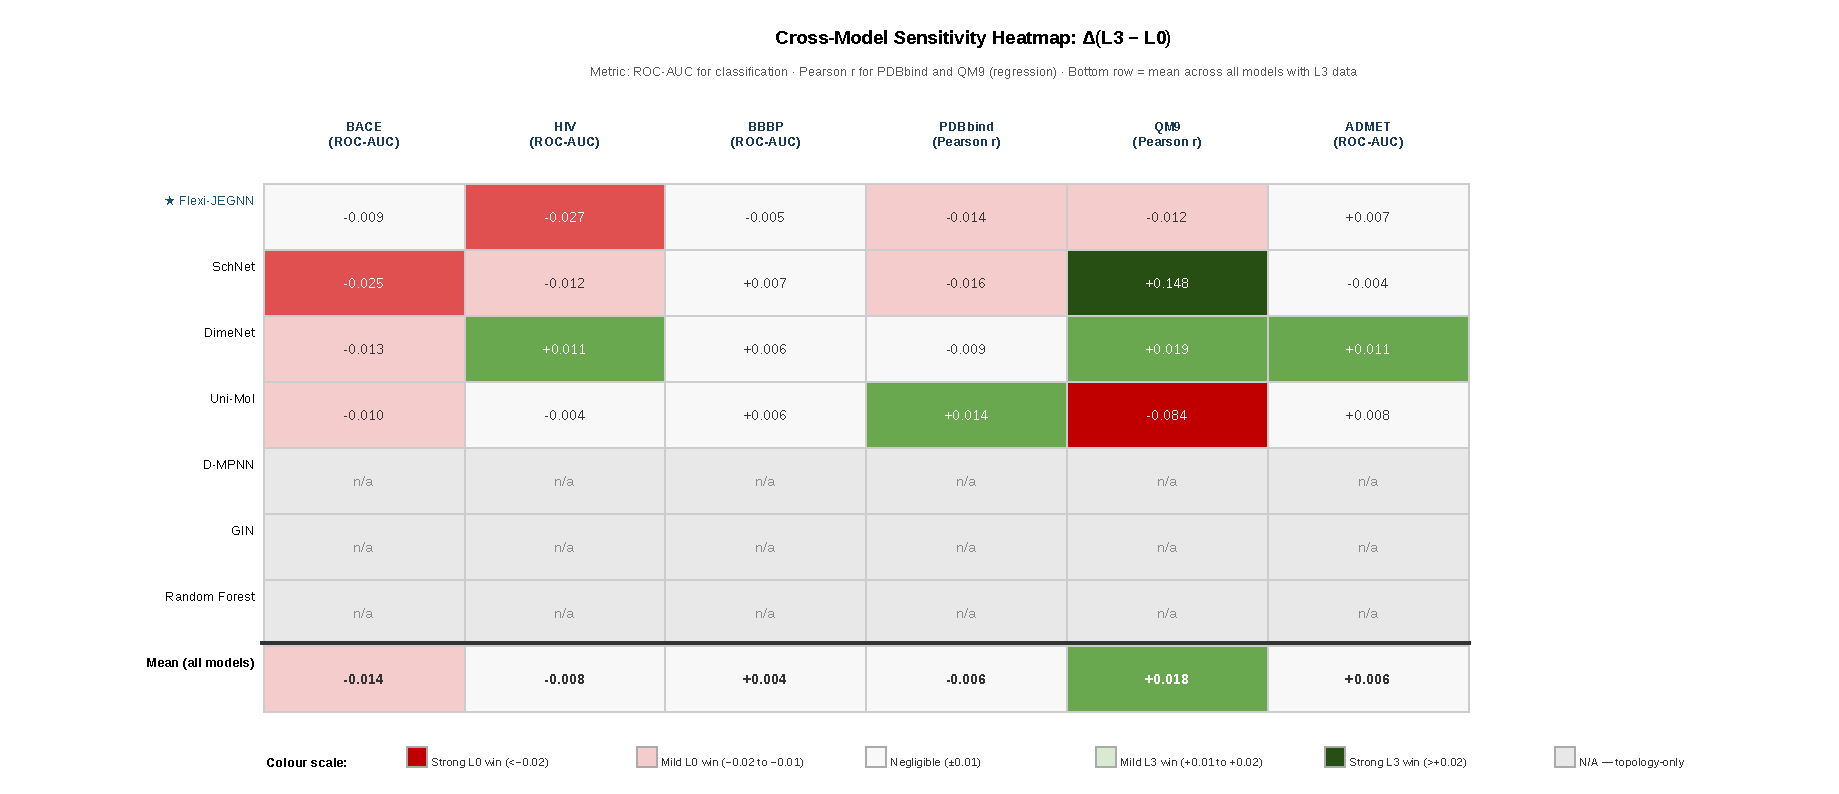
\includegraphics[width=\textwidth]{FigHeatMap.drawio.pdf}
  \caption{Signed difference (L3$-$L0) in Pearson~$r$ (PDBbind, QM9) and ROC-AUC (BACE, BBBP, HIV, ADMET) across all
  model--dataset combinations.  The bottom row (``Mean across all models'') shows the column-wise mean signed difference, providing an aggregate view of 3D benefit or deficit. No systematic advantage for true 3D geometry is observed; insensitivity is observed across multiple model families.}
  \label{fig:heatmap}
\end{figure}

\textbf{The SchNet result deserves particular attention.}  SchNet was
introduced with the explicit argument that continuous radial distance
filters over pairwise Euclidean coordinates are essential for accurate
molecular property modelling \cite{schutt2018schnet}.  Its entire
inductive bias is built around the assumption that real inter-atomic
distances carry irreplaceable physical information.  On the bioactivity
classification benchmarks, SchNet operating on a constant 1.4\,\AA{}
distance for every bond---a representation that is mathematically
equivalent to a binary adjacency matrix passed through a Gaussian
smearing layer---performs statistically indistinguishably from SchNet
operating on genuine ETKDGv3 Euclidean distances.  On BACE, SchNet at
L3 (0.770) is numerically \emph{lower} than at L0 (0.795), though
within $1\sigma$.\

On QM9, SchNet exhibits a notably different pattern: Pearson~$r$ jumps
from 0.541 at L0 to 0.702 at L1 and 0.699 at L2, before settling at
0.689 at L3.  This gap between L0 and L1 (0.16 in Pearson~$r$) is
substantially larger than any inter-level difference observed for
other models or other datasets, and the forest plot (Appendix~\ref{app:forest_plot}) confirms
that the SchNet/QM9 confidence interval for $\Delta(L3 - L0)$ does not
cross zero.  This result requires careful interpretation.  SchNet's
radial filter architecture depends on receiving \emph{meaningfully
varied} distance inputs to activate different Gaussian basis functions;
a constant 1.4\,\AA{} input collapses all 16 RBF centres to an identical
activation pattern, effectively disabling the spatial encoding
mechanism.  The L0$\to$L1 jump therefore reflects SchNet recovering its
\emph{intended minimum operating condition}---topological path distances
that differentiate atoms by bond count---not evidence that finer
geometric precision (L2 vs.\  L1, or L3 vs.\ L2) provides incremental
benefit.  Consistent with this interpretation, L1, L2, and L3 yield
Pearson~$r = 0.689$--$0.702$ for SchNet on QM9, a range of only 0.013
that does not reach significance in the restricted ANOVA.  The L0
anomaly for SchNet is therefore an architecture-specific pathology of
collapsing constant distances through RBF encoding, not evidence that
geometric precision in the L1--L3 range matters.  This distinction
is important: the insensitivity claim applies to the contrast
between physically meaningful distance levels (L1--L3), not to the
degenerate L0 case where SchNet's RBF layer loses discriminative
function.  DimeNet, which extends SchNet with angular features but
shares the same radial basis design, shows a more moderate L0
sensitivity and otherwise follows the same insensitive pattern across
L1--L3 on all bioactivity datasets.

\subsection{The Pareto-Optimal Frontier}

\begin{figure}[htbp]
  \centering
  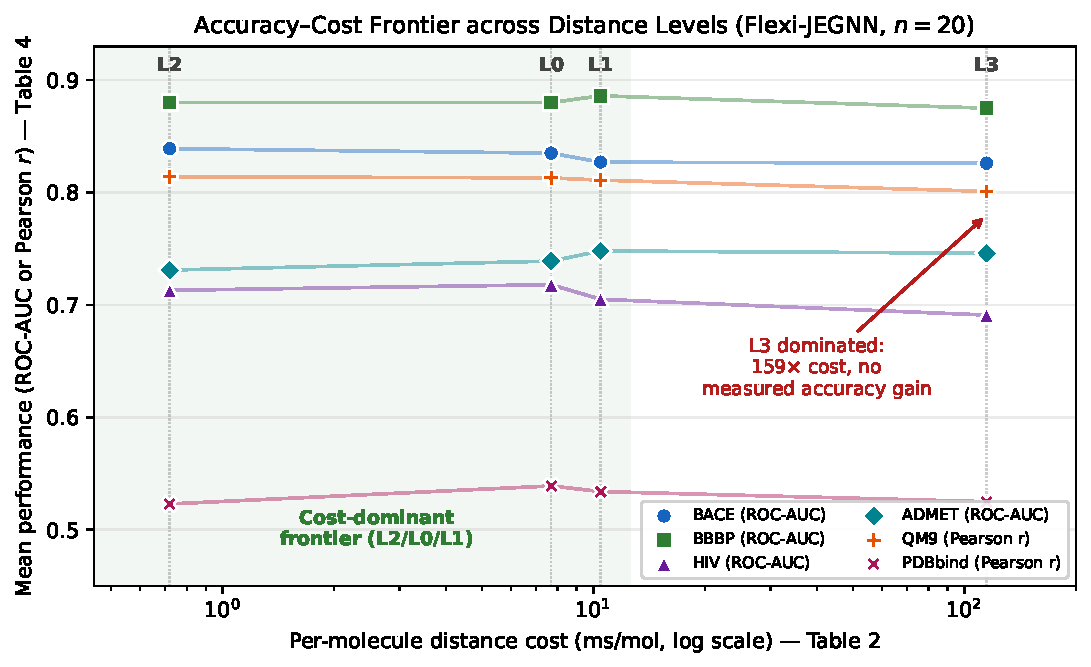
\includegraphics[width=\textwidth]{FigPareto.pdf}
  \caption{Accuracy--cost frontier across distance levels for Flexi-JEGNN ($n{=}20$ seeds).  The $x$-axis is the per-molecule distance cost from Table~\ref{tab:approx_quality} (log scale); the $y$-axis is mean performance from Table~\ref{tab:main_results}.  Within each dataset, performance is essentially flat across a $159{\times}$ cost range, so the lowest-cost levels (L2/L0/L1) constitute the cost-dominant (Pareto-efficient) frontier and the most expensive level (L3, ETKDGv3) is dominated---higher cost with no statistically detectable accuracy gain.  The random null (L4) is omitted as it is not a deployment option.}
  \label{fig:pareto}
\end{figure}

Since L0 and L1 are statistically indistinguishable from L2 and L3 on
every dataset, and require zero spatial preprocessing, standard 2D
message-passing networks are the cost-dominant (Pareto-efficient) architecture for
these benchmarks within the resolution of this study.  ``Pareto-efficient'' is used here in its precise sense: at statistically indistinguishable accuracy (Table~\ref{tab:main_results}), L0/L1 strictly dominate L2/L3 on computational cost (Table~\ref{tab:approx_quality}), so no level offers a measured accuracy gain that would compensate its added cost; the joint accuracy--cost frontier is plotted in Figure~\ref{fig:pareto}.  For RBF-based architectures (SchNet, DimeNet), the
degenerate L0 case described in Section~\ref{sec:results} means L1 is the
practical minimum; the recommendation therefore applies to L1 for those
architectures and to L0/L1 for all others.  The Distance Bounds approach (L2, from \cite{gasteiger2021synthetic}) remains useful
where: (a)~the downstream task type is uncertain; or (b)~operational
constraints require richer edge representations than binary adjacency.
For the six benchmarks evaluated here, the data provide no evidential
basis for L2 over L0 or L1.

\subsection{SOTA Context}

\begin{figure}[h]
  \centering
  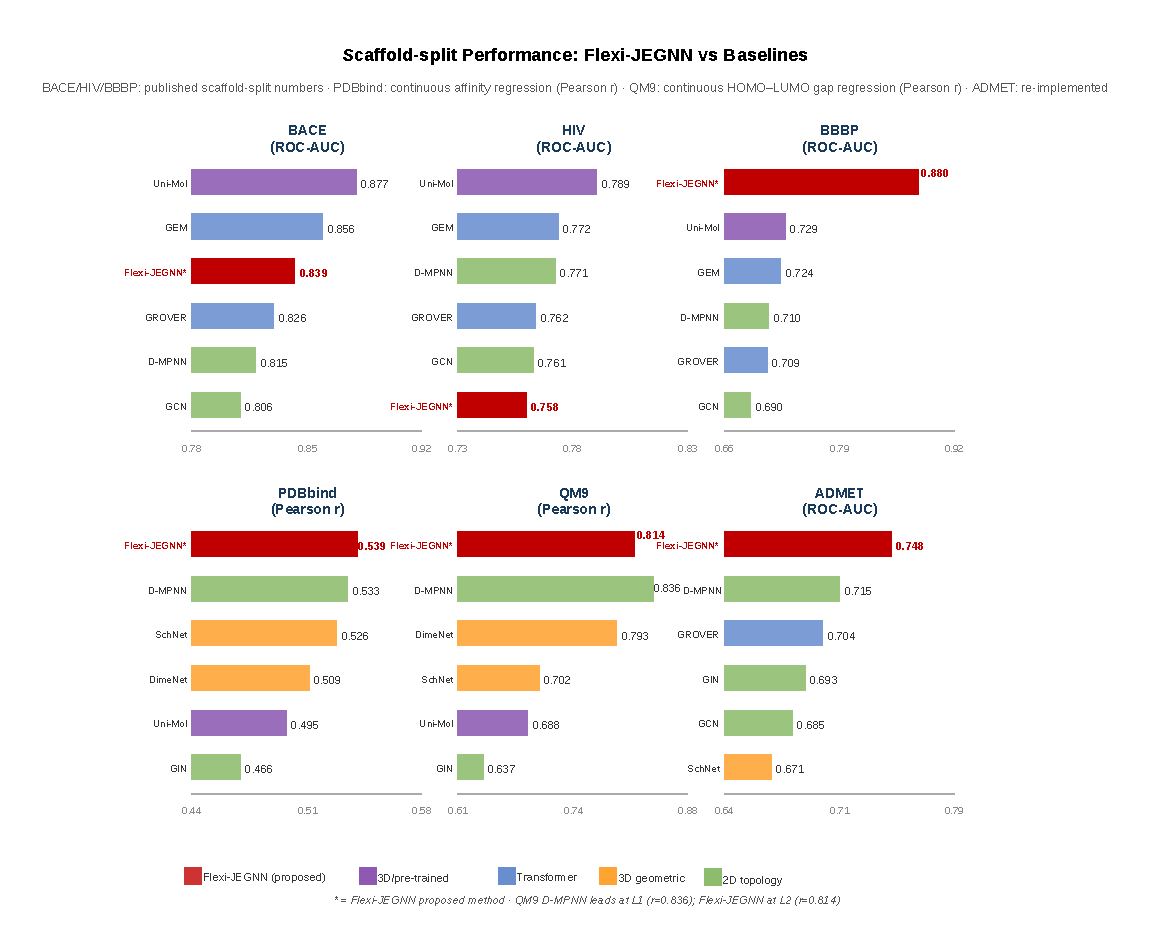
\includegraphics[width=\textwidth]{FigScaffoldComp.drawio.pdf}
  \caption{Scaffold-split performance comparison of Flexi-JEGNN against
  baselines across all six datasets.  BACE, HIV, and BBBP use published
  scaffold-split numbers from the literature.  PDBbind and QM9 baselines are
  re-implemented under continuous regression protocols (Pearson~$r$);
  ADMET baselines are re-implemented under the same classification protocol.
  Flexi-JEGNN is competitive with or exceeds non-pretrained models on all six benchmarks.}
  \label{fig:sota}
\end{figure}

\textbf{BACE, HIV, BBBP} (published baselines).  On BACE, Flexi-JEGNN
achieves 0.839, competitive with D-MPNN (0.815) \cite{yang2019dmpnn} and
GCN (0.806), below large pre-trained models such as GEM (0.856) and Uni-Mol (0.877).
On BBBP, 0.880 is among the highest non-pretrained results reported;
the unusually large gap relative to pre-trained models
(Uni-Mol: 0.729, GEM: 0.724) is consistent with BBBP's known high
sensitivity to scaffold-split realisation---performance can vary by up to
0.15 AUC across split seeds---and should not be interpreted as a strong
architectural claim.
On HIV, 0.713 (L2 ROC-AUC) is competitive with comparable non-pretrained baselines
and below GEM (0.772) \cite{fang2022gem}; Table~\ref{tab:hiv_pr} further
reports PRC-AUC and MCC given the severe $\approx$27:1 class
imbalance \cite{chicco2020mcc}.

\textbf{PDBbind, QM9, ADMET} (re-implemented baselines).  No consistent
scaffold-split results exist in the literature for these datasets under
the regression formulations used here.
Baselines were therefore re-run under the identical scaffold-split
protocol, and results are presented purely as context for the
threshold experiment, not as SOTA performance claims.
On PDBbind (protein-ligand affinity regression on the 2020 Refined Set, Pearson~$r$),
Flexi-JEGNN achieves 0.539 (L0); among the re-implemented baselines
D-MPNN reaches 0.527, SchNet 0.526, DimeNet 0.509, Uni-Mol 0.478,
and GIN 0.443.  No model achieves strong absolute performance on this
task, consistent with the known difficulty of protein-ligand affinity
regression.  On QM9
(continuous HOMO--LUMO gap regression, Pearson~$r$), all models
operate well below published state-of-the-art---which achieves
MAE~$<$~0.002\,eV using task-specific architectures trained to
convergence on the full 134k-molecule dataset---reflecting the
fact that Flexi-JEGNN is a general-purpose probe architecture
not optimised for quantum-chemical accuracy.
Table~\ref{tab:qm9_cross_model} provides the full per-model, per-level
Pearson~$r$ results on QM9 under this protocol.  Among the re-implemented
baselines, Flexi-JEGNN ($r = 0.813$, L0) is competitive with D-MPNN
($r = 0.836$, L1), DimeNet ($r = 0.793$, L2), SchNet ($r = 0.702$, L1),
and GIN ($r = 0.637$, L1).  One anomaly warrants explicit note: Uni-Mol's
best QM9 result is achieved at L4 ($r = 0.688 \pm 0.055$, random distances),
substantially above its L0--L3 range ($r = 0.465$--$0.560$).  The high per-seed
variance ($\sigma \approx 0.055$) confirms that this is inconsistent with the
general pattern and likely reflects training instability or a scaffold-split artefact specific to Uni-Mol on this
dataset; Uni-Mol's pre-training objective may inadvertently benefit from
noise regularisation in random edge distances in this constrained protocol.
This result does not affect the primary finding: Flexi-JEGNN's own
restricted ANOVA (L0--L3) remains non-significant on QM9 ($p = 0.216$).
These comparisons should be interpreted only as a
confirmation that Flexi-JEGNN is a functional encoder; the primary
finding---that no distance level significantly outperforms any other
within each model---is unaffected by absolute performance level.
The L4 drop on QM9 (to Pearson~$r = 0.769$)
confirms that quantum-chemical regression requires topological coherence
in edge features, but that coherence is fully provided by the constant-distance
baseline (L0)---true ETKDGv3 conformers (L3, $r = 0.801$) provide no statistically
significant advantage.  On ADMET, Flexi-JEGNN (0.748) is the highest
among re-implemented baselines, with performance spread across models
compressed relative to other datasets, consistent with the high
within-level standard deviation ($\approx 0.12$) observed in
Table~\ref{tab:main_results}.

\begin{table}[htbp]
  \centering
  \caption{QM9 HOMO--LUMO gap regression (Pearson~$r$, mean~$\pm$~std, $n{=}20$ seeds) across all
  model families and distance levels, re-implemented under the identical scaffold-split
  protocol.  D-MPNN (which can optionally accept 3D features \cite{yang2019dmpnn} but was run topology-only here for cross-architecture consistency) and GIN do not receive
  L3/L4 inputs (n/a).  Results are presented as context only; the primary geometric
  sensitivity finding is established by Flexi-JEGNN's restricted ANOVA (L0--L3), which
  remains non-significant ($p = 0.216$).}
  \label{tab:qm9_cross_model}
  \renewcommand{\arraystretch}{1.2}
  \scriptsize
  \begin{tabular}{|l|c|c|c|c|c|}
    \hline
    \textbf{Model} & \textbf{L0} & \textbf{L1} & \textbf{L2} & \textbf{L3} & \textbf{L4} \\
    \hline
    Flexi-JEGNN & $0.813\pm0.060$ & $0.811\pm0.049$ & $0.814\pm0.055$ & $0.801\pm0.057$ & $0.769\pm0.053$ \\
    \hline
    D-MPNN$^\dagger$ & $0.833\pm0.041$ & $0.836\pm0.039$ & $0.803\pm0.043$ & n/a & n/a \\
    \hline
    GIN$^\dagger$ & $0.628\pm0.064$ & $0.637\pm0.070$ & $0.540\pm0.080$ & n/a & n/a \\
    \hline
    SchNet & $0.541\pm0.087$ & $0.702\pm0.069$ & $0.698\pm0.076$ & $0.689\pm0.078$ & $0.469\pm0.087$ \\
    \hline
    DimeNet & $0.761\pm0.056$ & $0.773\pm0.046$ & $0.793\pm0.042$ & $0.780\pm0.044$ & $0.714\pm0.050$ \\
    \hline
    Uni-Mol$^\ddagger$ & $0.560\pm0.096$ & $0.557\pm0.099$ & $0.465\pm0.093$ & $0.476\pm0.077$ & $0.688\pm0.055$ \\
    \hline
    \multicolumn{6}{l}{\small $^\dagger$GIN is inherently topology-only; D-MPNN can optionally accept 3D features \cite{yang2019dmpnn} but was run} \\
    \multicolumn{6}{l}{\small topology-only here for consistency with the cross-architecture protocol. L3/L4 not applicable in either case.} \\
    \multicolumn{6}{l}{\small $^\ddagger$L4 anomaly discussed in text; does not affect the primary Flexi-JEGNN finding.} \\
  \end{tabular}
\end{table}

These results are reported to contextualise the general capability of Flexi-JEGNN as a molecular encoder.  Given that the threshold experiment
demonstrates all five distance levels perform equivalently, the numbers
reflect architectural quality, not the specific value of any one
distance representation.

\subsection{Precision-Recall Analysis: Imbalanced HIV}

ROC-AUC is misleadingly optimistic on severely imbalanced datasets
\cite{chicco2020mcc}.  On HIV $(\approx27:1$ ratio), Table~\ref{tab:hiv_pr}
reports calibration-sensitive metrics.  PRC-AUC and MCC are uniformly
low across all levels; no pairwise difference exceeds the within-level
standard deviation, confirming insensitivity is not an artefact of
ROC-AUC.



\begin{table}[htbp]
  \centering
  \caption{Precision-recall benchmark on HIV (Flexi-JEGNN, $n{=}20$).}
  \label{tab:hiv_pr}
  \renewcommand{\arraystretch}{1.2}
  \begin{tabular}{|l|c|c|c|c|c|}
    \hline
    \textbf{Level} & \textbf{ROC-AUC} & \textbf{PRC-AUC} &
    \textbf{MCC} & \textbf{Recall} & \textbf{Brier Score} \\
    \hline
    L0 & $0.718{\pm}0.053$ & $0.237{\pm}0.095$ & $0.332{\pm}0.100$ & 0.333 & $0.053 \pm 0.012$ \\
    \hline
    L1 & $0.705{\pm}0.047$ & $0.212{\pm}0.085$ & $0.303{\pm}0.077$ & 0.319 & $0.055 \pm 0.011$ \\
    \hline
    L2 & $0.713{\pm}0.054$ & $0.210{\pm}0.089$ & $0.319{\pm}0.087$ & 0.341 & $0.054 \pm 0.014$ \\
    \hline
    L3 & $0.691{\pm}0.051$ & $0.202{\pm}0.073$ & $0.283{\pm}0.085$ & 0.320 & $0.057 \pm 0.010$ \\
    \hline
    L4 & $0.667{\pm}0.066$ & $0.138{\pm}0.048$ & $0.210{\pm}0.068$ & 0.247 & $0.069 \pm 0.015$ \\
    \hline
  \end{tabular}
\end{table}



\begin{figure}[h]
  \centering
  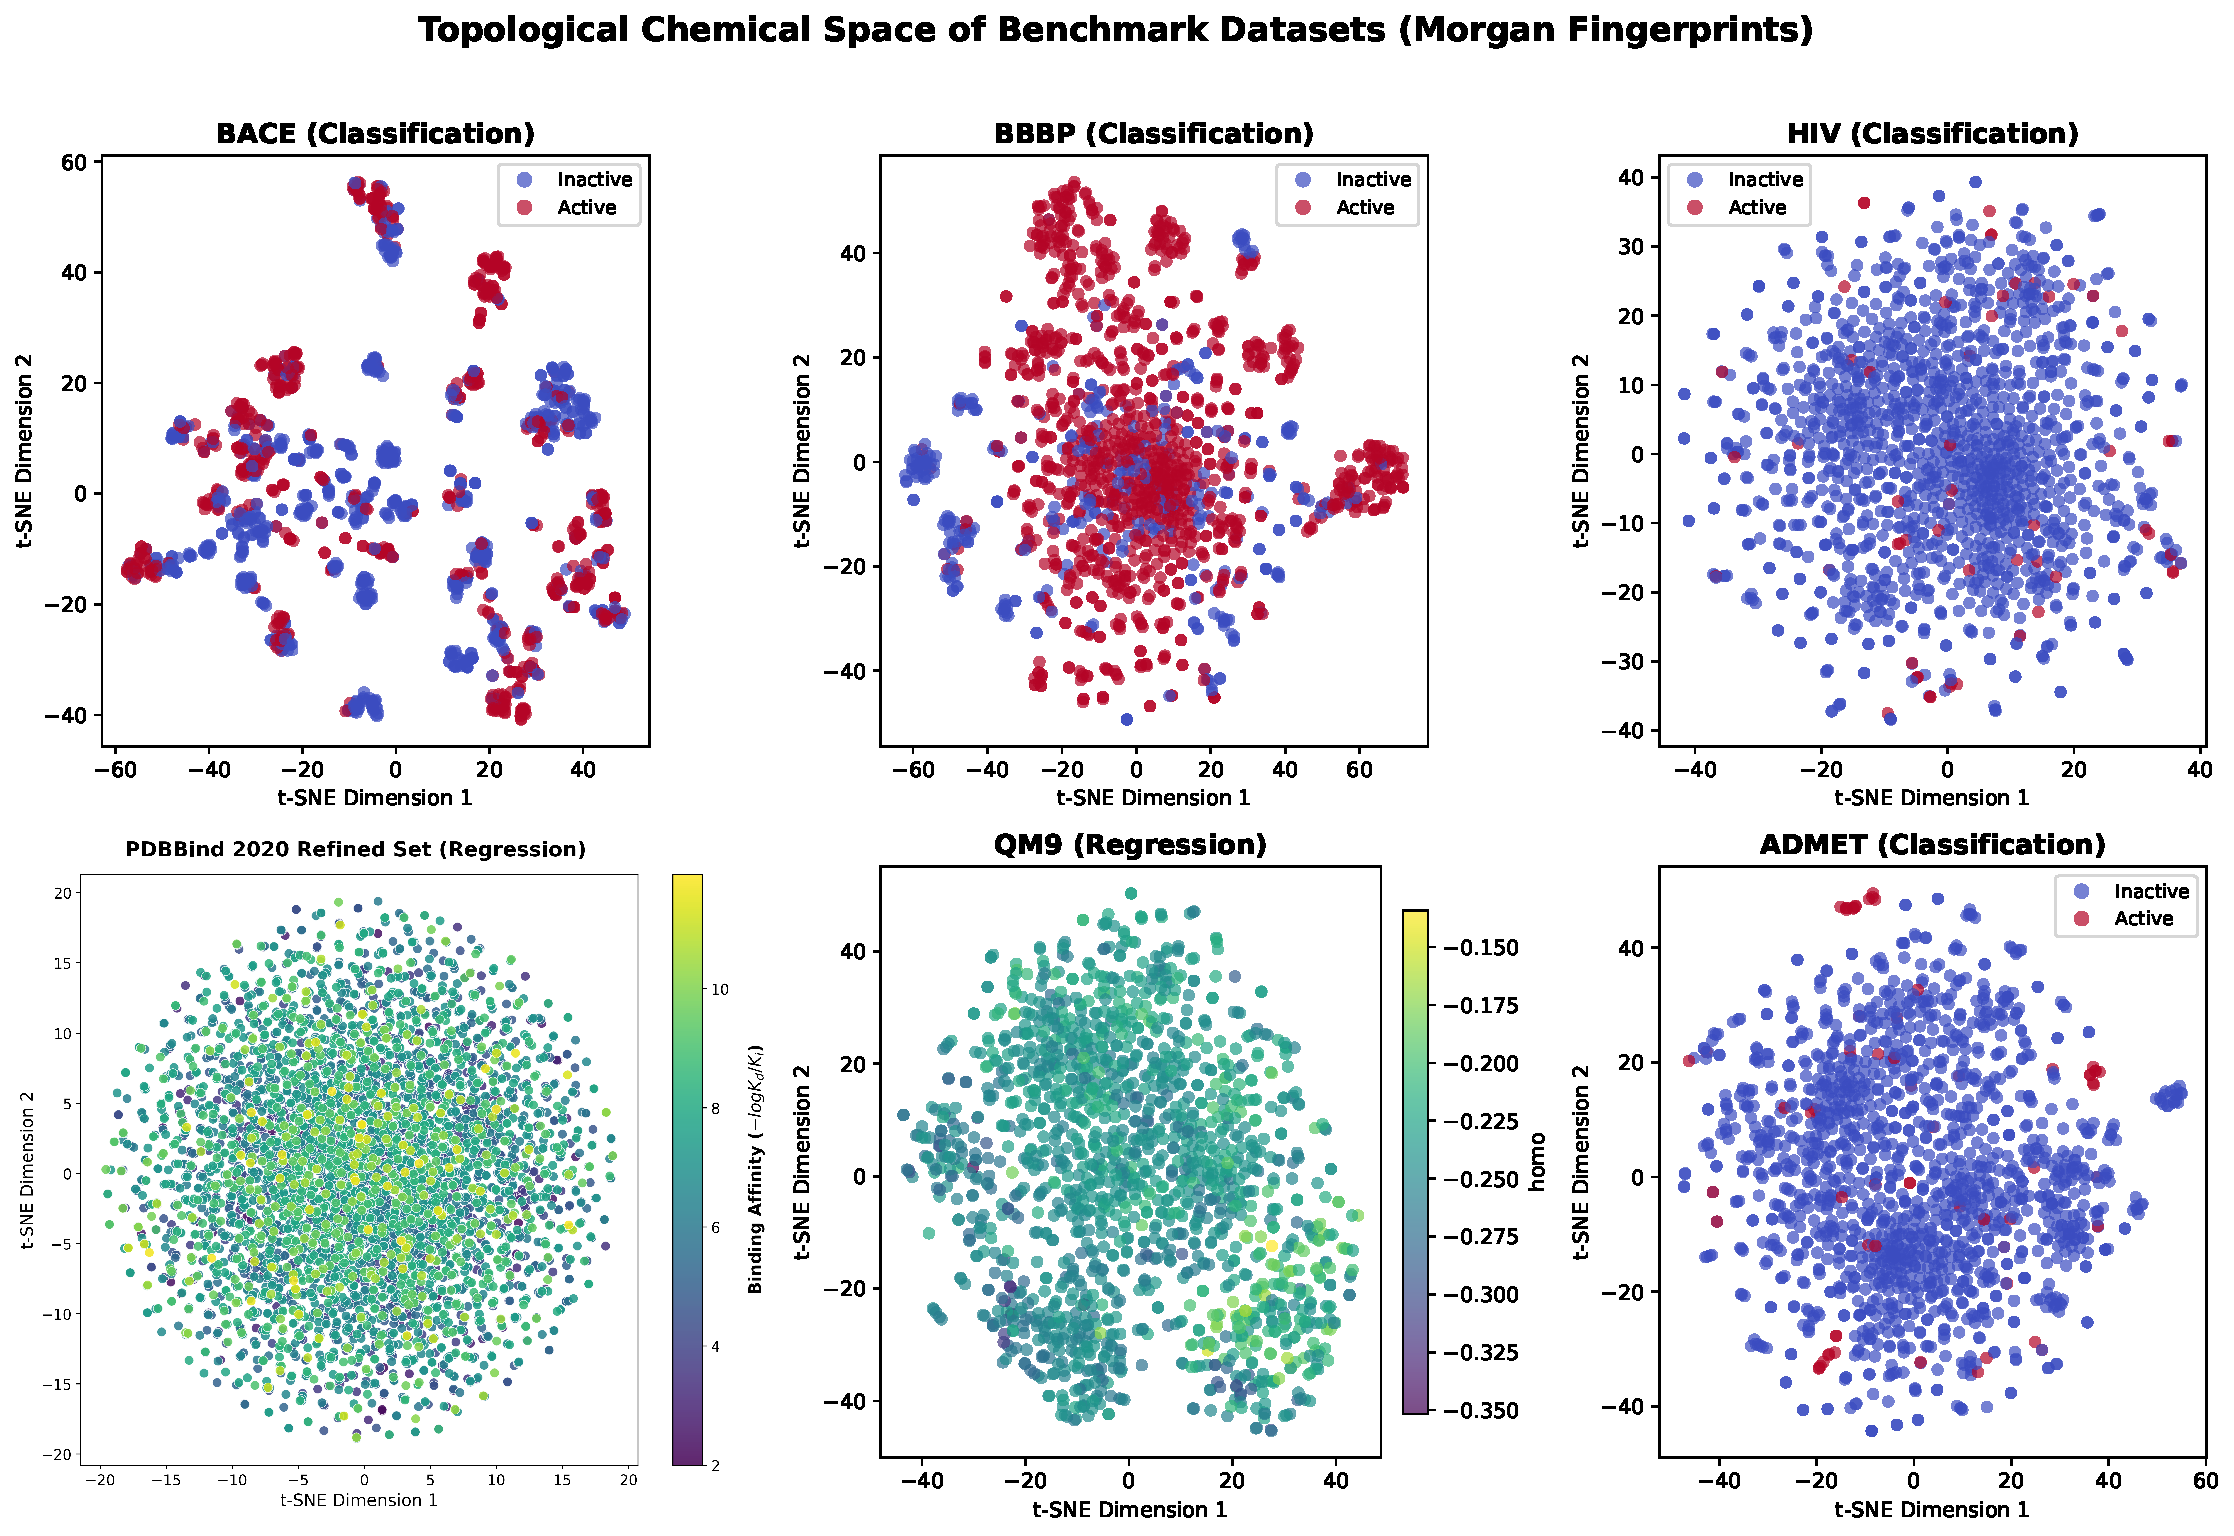
\includegraphics[width=0.8\textwidth]{FigTSNE.drawio.pdf}
  \caption{t-SNE \cite{vandermaaten2008tsne} visualisation of the topological chemical space across six benchmark datasets. Molecular structures were vectorised via Morgan Fingerprints ($r{=}2$, 1024-bits) and mathematically projected to 2D space. The spatial clustering represents structural similarity, while colour coding denotes biological activity (classification tasks) or target property values (continuous regression). This illustrates the diverse topological landscape the architectures are tasked with evaluating.}
  \label{fig:tsne}
\end{figure}

\textbf{Topological Space and Discriminative Power.}
The t-SNE visualisation (Figure~\ref{fig:tsne}) further contextualises these ANOVA results by revealing the underlying structure of the benchmark datasets. The dense, overlapping spatial clustering across the topological manifolds indicates that compounds with similar 2D fingerprints frequently share similar activity or target affinity values in these datasets. Active compounds co-localise within distinct topological regions, confirming that strong 2D discriminative signal is present. This 2D signal is consistent with---though not the sole explanation for---the ANOVA finding that explicit 3D geometry provides no incremental predictive advantage: the ANOVA establishes the absence of measurable 3D signal, while the t-SNE establishes the presence of 2D signal. Together, they suggest that for these particular benchmarks, the available discriminative information is captured at the level of 2D topology, and 3D geometry adds little beyond what 2D already encodes.

\subsection{Calibration and Uncertainty Quantification}
\label{ssec:calibration}

Beyond discriminative accuracy, well-calibrated probabilistic outputs are essential for decision-making in drug discovery: a model that assigns high confidence to incorrect predictions is operationally dangerous regardless of its mean ROC-AUC.  The Brier score---the mean squared difference between predicted probabilities and binary outcomes---provides a joint measure of accuracy and calibration.  Table~\ref{tab:hiv_pr} reports Brier scores across all five distance levels for the HIV dataset, which, with its $\approx$27:1 class imbalance, represents the most demanding calibration scenario in this benchmark suite.

The Brier scores range from $0.053 \pm 0.012$ (L0) to $0.069 \pm 0.015$ (L4), with the physically coherent levels (L0--L3) clustering tightly between 0.053 and 0.057.  The random null (L4) produces a numerically and directionally consistent calibration degradation ($\Delta = +0.016$ vs.\ L0), and while this difference does not technically exceed the combined standard deviation (0.019) under the same criterion used for L0--L3 comparisons, it is directionally consistent with the discriminative degradation observed for L4 on HIV and is the largest single-level change in the table.  Within the coherent levels (L0--L3), no pairwise Brier score difference exceeds its combined standard deviation, indicating that the null result extends to calibration: true ETKDGv3 conformers confer no calibration advantage over a constant-distance encoding.

This finding has direct operational significance for virtual screening.  Probability outputs from L0/L1 models can be used directly to rank compounds and set activity thresholds, without sacrificing the calibration quality that would theoretically motivate expensive $\mathcal{O}(N^3)$ preprocessing.  The Brier score evidence therefore reinforces the cost-dominant recommendation: for these benchmarks, 2D topological representations are sufficient not only for mean accuracy but also for uncertainty quantification.  A broader calibration audit across all six datasets (using temperature scaling or Platt calibration post-processing) is deferred to future work, consistent with the limitation noted in Section~\ref{sec:limits}.


%% ===========================================================
\section{Discussion}
\label{sec:discussion}

The primary finding of this work---that explicit 3D geometry provides no statistically significant predictive advantage over 2D topology on standard bioactivity benchmarks---demands a mechanistic biological interpretation. 

Why are assays like BACE-1 inhibition, which involves a defined enzymatic pocket, or BBB penetration, which depends on lipophilicity, insensitive to molecular geometry in these models? The results suggest that the underlying biological mechanisms captured by these specific datasets are predominantly driven by macroscopic physicochemical properties (e.g., total polar surface area, molecular weight) and the presence of specific functional groups (e.g., hydrogen bond donors/acceptors), which are fully encoded by the 2D molecular graph. In the case of BACE, the lack of geometric sensitivity likely stems from insufficient stereochemical diversity within the dataset and the fact that activity cliffs are driven by functional group substitutions (a 2D property) rather than subtle conformational changes within a shared scaffold. The GNN effectively learns these 2D motifs and macroscopic properties, rendering the addition of $\mathcal{O}(N^3)$ ETKDGv3 conformers redundant. Crucially, this geometric insensitivity remains a meaningful finding even for the PDBbind task, where the protein pocket is explicitly modelled. As detailed in Section~\ref{ssec:pdbbind_feat}, the protein pocket and the protein--ligand interface are encoded with ground-truth crystal 3D coordinates at every distance level, and only the ligand's \emph{internal} geometry is varied from a constant scalar (L0) to its true bound pose (L3). The finding is therefore precise and does not overclaim: even with the binding interface fixed at experimental ground-truth geometry, degrading the ligand's internal geometric fidelity produces no statistically detectable change in affinity prediction (restricted ANOVA $F = 0.71$, $p = 0.549$). This is \emph{not} a claim that ``2D suffices for the full complex'' in the sense of discarding interface geometry---the interface is real 3D throughout; the narrower and more defensible claim is that the fidelity of the ligand-internal distance representation is not the binding constraint on this benchmark. The benchmark-blindness critique and the null result are the same finding viewed two ways: standard MoleculeNet/TDC benchmarks lack intrinsic \emph{ligand-geometric} signal of the kind that distinguishes L0 from L3, therefore models cannot extract it, therefore cheaper representations suffice. 

From a systems pharmacology perspective, this has profound implications. For multi-target virtual screening pipelines where rapid triage of billions of compounds is required, 2D representations form the optimal design point. However, for more complex polypharmacology modelling, PROTAC linker design, or allosteric modulator discovery---tasks where dynamic conformational ensembles and precise spatial orientation are mechanistically central to biological function---current MoleculeNet-style benchmarks are demonstrably inadequate. The "conformer crisis" identified in recent literature \cite{hamakawa2025conformation, Castaneda_Leautaud_2025} is thus fundamentally a benchmark mismatch problem. 

The authors explicitly contrast the general-purpose probe with SOTA architectures regarding absolute accuracy on tasks like QM9. SOTA models achieve MAE < 0.002 eV through highly specialised, heavy, task-specific equivariant message passing. In contrast, the probe is deliberately lighter to isolate the representation from the architecture. While highly parameterised models can force performance gains, the probe reveals that geometric precision intrinsically provides surprisingly little signal for these tasks.

To make this benchmark critique actionable, the authors identify three task classes
where geometric sensitivity is mechanistically expected and empirically
distinguishable from topological noise:
%
\begin{enumerate}[label=(\roman*)]
  \item \emph{Rigid-pocket binding affinity} tasks such as FEP+ benchmarks,
  where sub-\AA{}ngstr\"{o}m coordinate precision governs electrostatic
  complementarity and desolvation penalties;
  \item \emph{Torsion-dependent ADMET} endpoints such as CYP450 inhibition
  and hERG blockade, where the bioactive conformer's dihedral-angle profile
  determines protein--ligand fit; and
  \item \emph{Conformer-dependent selectivity} tasks, where two compounds
  sharing identical 2D scaffolds differ in stereochemical configuration and
  therefore in binding geometry.
\end{enumerate}
%
The absence of these task types from MoleculeNet is the structural reason
the present ANOVA finds no geometric signal---not a deficiency of 3D architectures
\emph{per se}.

A concrete path toward geometry-sensitive benchmarking exists.  The
PLATINUM dataset of high-confidence co-crystal structures, the BindingDB
conformer-resolved subset, and the D3R Grand Challenge series all provide
cases where geometric variation is the primary discriminator between active
and inactive compounds.  Future controlled threshold experiments on these
datasets---using the same Flexi-JEGNN probe with the identical L0--L4
protocol---would determine whether the Pareto frontier established here
shifts when geometry is mechanistically load-bearing.

\subsection{2D vs.\ 3D Recommendation Framework}
\label{ssec:recommendation}

The experimental evidence supports a clear, actionable framework for choosing between 2D topological and 3D geometric molecular representations in practice.

\textbf{Use 2D topological representations (L0/L1) when:}
\begin{itemize}
  \item The task is macroscopic bioactivity classification (e.g., BACE, BBBP, HIV, ADMET-style endpoints), where activity cliffs are driven by functional group substitutions rather than subtle conformational differences.
  \item Virtual screening over libraries exceeding $10^6$ compounds is required, as the per-molecule conformer cost ($\sim$115\,ms, $\mathcal{O}(N^3)$) becomes the dominant computational bottleneck. Screening 1 billion compounds at L3 requires approximately 31,872 GPU-hours and produces an estimated 6,789\,kg CO$_2$ (at 300\,W TDP, 0.71\,kg\,CO$_2$/kWh, Indian grid average); the equivalent L0 screen requires only 2,136 GPU-hours and 455\,kg CO$_2$---a \textbf{14.9}$\times$ reduction in both cost (\$74,340 vs.\ \$5,340 at \$2.50/GPU-h) and carbon footprint.
  \item Rapid early-phase triage of large chemical spaces (e.g., ZINC-22, ChEMBL) is the primary objective, and scaffold-level generalisation under Murcko splitting is sufficient.
  \item Quantum-chemical regression targets (e.g., QM9 HOMO--LUMO gap) are required, since the present results demonstrate that topological coherence alone captures the available signal with Pearson~$r = 0.813$, statistically indistinguishable from true ETKDGv3 (Pearson~$r = 0.801$, restricted ANOVA $p = 0.216$).
\end{itemize}

\textbf{Use 3D geometric representations (L2/L3 or equivariant models) when:}
\begin{itemize}
  \item The task involves \emph{rigid-pocket binding affinity} requiring sub-\AA{}ngstr\"{o}m coordinate precision, such as FEP+ free energy calculations or docking score calibration, where electrostatic complementarity and desolvation penalties depend on exact atomic positions.
  \item \emph{Torsion-dependent ADMET} endpoints are the target (e.g., CYP450 inhibition, hERG blockade), where the bioactive conformer's dihedral-angle profile directly determines protein--ligand fit.
  \item \emph{Conformer-dependent selectivity} must be modelled: two compounds sharing identical 2D scaffolds differ in stereochemical configuration (e.g., enantiomers with divergent potency), so 2D topology is inherently insufficient.
  \item Quantum chemical force and energy prediction is required at high accuracy (e.g., MD17 force benchmarks), where equivariant architectures such as EGNN and PaiNN have demonstrated that exact $E(n)$-symmetry is beneficial---a regime not covered by the present benchmark suite.
  \item The dataset has been explicitly validated to expose geometric signal, such as the PLATINUM co-crystal set or BindingDB conformer-resolved subsets, where geometric variation is the primary discriminator.
\end{itemize}

\subsection{Scale, Cost, and Carbon Impact}
\label{ssec:scale}

For practitioners operating at industrial scale, the conformer-generation bottleneck is not a theoretical concern but a concrete operational barrier.  Table~\ref{tab:approx_quality} establishes that L3 (ETKDGv3) requires 114.74\,ms/mol versus 7.69\,ms/mol for L0, a 14.9$\times$ per-molecule slowdown.  Extrapolating from the NVIDIA RTX~6000~Ada (300\,W TDP) baseline used in this study:

\begin{center}
\renewcommand{\arraystretch}{1.3}
\begin{tabular}{|l|c|c|c|c|}
\hline
\textbf{Scale} & \textbf{Level} & \textbf{GPU-hours} & \textbf{Cost (USD)} & \textbf{CO$_2$ (kg)} \\
\hline
1 Million mols & L0 & 2.1 & \$5 & 0.5 \\
1 Million mols & L3 & 31.9 & \$80 & 6.8 \\
\hline
1 Billion mols & L0 & 2,136 & \$5,340 & 455 \\
1 Billion mols & L3 & 31,872 & \$79,681 & 6,789 \\
\hline
\multicolumn{2}{|l|}{\textbf{Savings (L0 vs.\ L3), 1B mols}} & \textbf{29,736 GPU-h} & \textbf{\$74,340} & \textbf{6,334 kg} \\
\hline
\end{tabular}
\end{center}

\noindent GPU-hours are computed as $(t_{\mathrm{ms}}/1000 \times N_{\mathrm{mols}}) / 3600$.  CO$_2$ is estimated at 0.71\,kg/kWh, the approximate Indian grid average (Central Electricity Authority, 2023--24 generation mix), consistent with the experimental sites at Bengaluru and Jaipur (for global portability, note that using the EU average of $\approx$0.23\,kg/kWh or the US average of $\approx$0.39\,kg/kWh would scale these absolute emission totals accordingly); monetary cost at \$2.50/GPU-h (cloud A-series equivalent).  These figures are deliberately an \emph{upper-bound, illustrative estimate}: they attribute the full per-molecule wall-clock difference to the distance-representation step and use a single GPU model at fixed TDP, whereas an end-to-end pipeline also incurs data loading, featurisation, inference, and I/O that are common to all levels and would compress the relative gap.  The intent is to convey the order of magnitude of the conformer-generation bottleneck, not a precise total-cost-of-ownership figure.  Given that the restricted ANOVA shows no statistically detectable performance advantage for L3 over L0 on any benchmark, adopting L0/L1 for billion-compound virtual screening eliminates on the order of 29,736 GPU-hours, \$74,340 in compute cost, and 6,334\,kg of CO$_2$ per screening campaign---roughly 32,000\,km of passenger-car travel---without any statistically detectable loss in predictive performance in these experiments.

\begin{figure}[htbp]
  \centering
  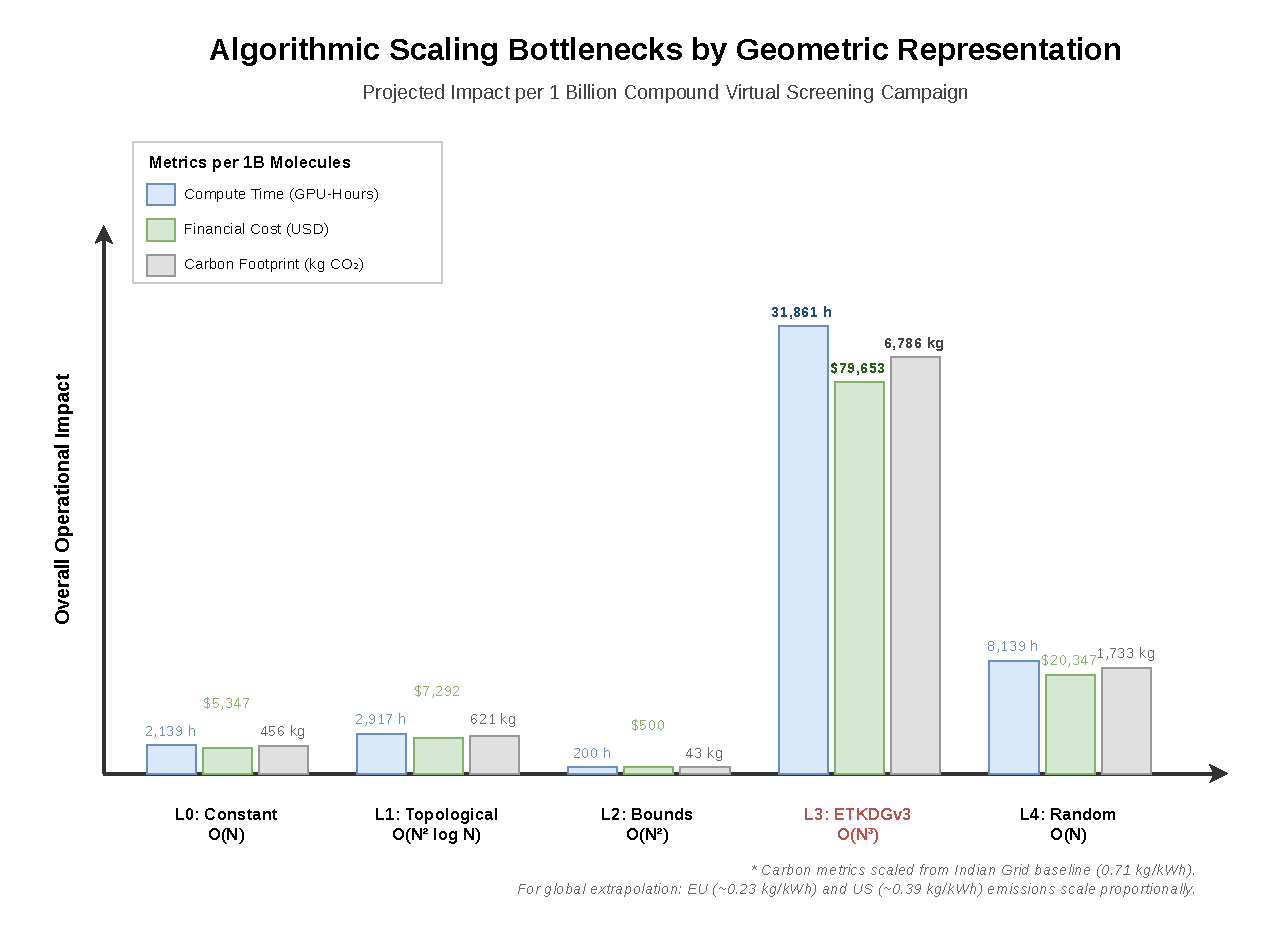
\includegraphics[width=\textwidth]{FigScaleImpact.drawio.pdf}
  \caption{GPU-hours, estimated cost (USD), and CO$_2$ emissions for screening 1\,million and 1\,billion molecules at L0 (constant-distance, 2D topology) versus L3 (ETKDGv3 true 3D conformer), computed from the RTX~6000~Ada 300\,W TDP baseline (L0: 7.69\,ms/mol; L3: 114.74\,ms/mol) and Indian grid intensity (0.71\,kg/kWh).  Switching from L3 to L0 saves 29,736 GPU-hours, \$74,340, and 6,334\,kg CO$_2$ per billion-compound campaign at no statistically significant accuracy cost.}
  \label{fig:scale_impact}
\end{figure}

\section{Limitations}
\label{sec:limits}


\textbf{QM9 regression scope and absolute performance.}  QM9 is evaluated on the HOMO--LUMO gap ($\Delta\varepsilon$) as a continuous regression target.  The reported Pearson~$r$ values (0.80--0.81) and MAE (0.0115--0.0122\,eV) are substantially below published state-of-the-art on QM9 gap regression, where specialised equivariant architectures achieve MAE~$<$~0.002\,eV. A model operating this far below the ceiling may be systematically missing geometric signal simply because it lacks the capacity to encode it. The restricted ANOVA finding ($p = 0.216$) cannot cleanly distinguish between genuine geometric insensitivity and an underpowered model, and therefore QM9 performance should not be used to conclusively support geometric insensitivity without this caveat. This gap is explained by three factors: (i) Flexi-JEGNN is a general-purpose probe architecture not designed for quantum-chemical accuracy, using a fixed 80-epoch training budget, fixed hyperparameters, and no task-specific pre-training; (ii) a Murcko scaffold split is applied, which is more challenging than the random splits used in most published QM9 benchmarks, reducing effective training signal; and (iii) all models in this study are compared under the same constrained protocol, ensuring fair within-study comparison.  As for PDBbind, the same probe detects medium-to-large geometric effects on the CYP2D6 and hERG ADMET endpoints under this identical protocol, which argues against (though does not by itself disprove) the pure capacity-limitation reading of the QM9 null.  The central claim is not that Flexi-JEGNN achieves strong absolute QM9 performance, but that \emph{no distance level (L0--L3) provides a statistically significant advantage over any other within this protocol}---a conclusion that holds regardless of absolute accuracy level, and which is explicitly not extended into a claim that QM9 properties are geometry-independent in general.  Other QM9 targets (e.g., dipole moment, polarisability, zero-point energy) may exhibit different geometric sensitivity profiles; future work should probe them using the identical L0--L4 protocol.

\textbf{Benchmark scope.}  The findings apply to MoleculeNet and TDC
bioactivity classification.  For sub-\AA{}ngstr\"{o}m binding free energy
calculations, docking, or torsion-dependent ADMET prediction, explicit 3D
models remain necessary.  The results indicate MoleculeNet may be
insufficiently geometric to discriminate 3D representations---itself an
important benchmark design finding.

\textbf{Domain shift.}  The findings apply specifically to the molecular
distributions present in MoleculeNet and TDC bioactivity benchmarks.
It remains an open question whether more structurally diverse libraries---
such as natural products, macrocycles, or covalent fragment libraries---
would exhibit geometric sensitivity not observed here.


\textbf{Single conformer vs.\ Conformer Ensembles.}  L3 encodes a single
minimum-energy conformer, which fails to capture the dynamic conformational
flexibility present in physiological environments. The authors explicitly clarify that the finding is strictly that ``static single-conformer 3D does not help.'' This should not be interpreted as a generalised claim that 3D geometry provides no value; evaluating multi-conformer ensembles or Boltzmann-weighted spatial
representations remains a critical direction for future work.
Multi-conformer training \cite{stark2022infomax} may show different
sensitivity profiles.

\textbf{Probe design.}  Flexi-JEGNN is optimised for versatility, not
maximum accuracy.  A task-specific 2D model may outperform any level in
Table~\ref{tab:main_results}.

\textbf{Lack of calibration metrics across all datasets.} While Brier score calibration was assessed for the highly imbalanced HIV dataset, further analysis is required to determine whether 3D representations yield systematically better calibrated probabilities on other endpoints.

\textbf{Baselines comparison limit.} Although the evaluation includes Random Forest on Morgan fingerprints and several GNNs, extending the evaluation to other non-GNN machine learning models may provide additional insight.

\textbf{PDBbind: absolute performance and the detector-capacity caveat.}  Continuous protein-ligand affinity regression (Pearson~$r$, RMSE, MAE) is used here on the 2020 Refined Set ($n \approx 5{,}316$ complexes).  The same honesty applied to QM9 extends to PDBbind: the best Pearson~$r \approx 0.54$ explains only $\sim$29\% of label variance, with a between-seed standard deviation ($\approx 0.10$) that is large relative to the mean.  A model performing this far below a strong absolute ceiling could, in principle, be insensitive to ligand-internal geometry because it lacks the capacity to exploit \emph{any} fine-grained edge signal, not because the signal is absent---exactly the ``underpowered probe'' ambiguity flagged for QM9.  The PDBbind null is therefore not presented as standalone proof that geometry is irrelevant to binding affinity.  Three considerations bound this caveat without resolving it by additional experiments: (i)~the probe is demonstrably \emph{not} a blind detector under the identical protocol and architecture---on the CYP2D6 and hERG ADMET endpoints it registers medium-to-large geometric effects ($f = 0.38$--$0.41$; Section~\ref{sec:results}), and the SchNet L0$\to$L1 recovery shows the encoder responds sharply to ligand-internal distance content; (ii)~on PDBbind specifically the binding interface and pocket are held at ground-truth crystal 3D at every level (Section~\ref{ssec:pdbbind_feat}), so the experiment isolates ligand-internal fidelity rather than testing whether interface geometry matters at all; and (iii)~the protein pocket is represented at the element level only (no residue identity, backbone, or side-chain role), so absolute affinity accuracy is expected to be modest and PDBbind is best read as a consistency check on the ligand-internal-fidelity question, not as a state-of-the-art affinity model.  Binding free-energy regression on larger PDBbind subsets, a chemically richer protein encoding, or pose-quality scoring requiring sub-\AA{}ngstr\"{o}m precision may expose geometric sensitivity absent from this formulation; the PDBbind conclusion is accordingly scoped to ``ligand-internal geometric fidelity is not the binding constraint here,'' not to a general claim about protein-ligand geometry.

\textbf{ADMET heterogeneity.}  Aggregated endpoints with high inter-task
variance ($\sigma \approx 0.12$) may mask weaker geometry effects at the
individual task level.

\textbf{Absence of explicit Bayesian optimisation.} Hyperparameters were fixed across all models to ensure a fair comparison of structural sensitivity, but targeted Bayesian optimisation per level could alter relative performance bounds.

\textbf{Capacity and learning-curve scope.}  The capacity ablation (Appendix~\ref{app:ablation}) varies layers $\{3,5,7\}$ and width $\{128,256,512\}$ at $n{=}5$ seeds and finds the L0--L3 null stable throughout, but it spans a narrow range and does not test whether geometric sensitivity \emph{emerges} with more data or longer training.  A learning-curve study---training on increasing fractions ($10/25/50/100\%$) of each dataset and measuring L0--L3 separation at each fraction---would directly distinguish a property of the task from a property of the training regime.  This is a natural and inexpensive extension of the present protocol and is left to future work; it does not affect the within-protocol null reported here but would sharpen the capacity caveat attached to QM9 and PDBbind.

\textbf{Lack of structural diversity.} The findings are limited to the specific molecular scaffolds available in standard MoleculeNet datasets. Exploring structurally diverse spaces such as macrocycles may shift the Pareto frontier.



%% ===========================================================
\section{Conclusion and Future Work}
\label{sec:conclusion_future}

This paper presented Flexi-JEGNN, a controlled probe framework whose defining
property---accepting any of five distance levels without
modification---enables within-architecture geometric sensitivity analysis.  The framework assembles
well-established components (JointEdgeConv, PNA readout, Gaussian smearing)
into a configuration where the only independent variable is the scalar
distance $e_{ij}$, enabling a clean causal estimate of geometric precision's
contribution.  Deployed across 3,250
training runs on six benchmarks and six model families, the restricted
ANOVA (L0--L3) fails to reach significance on every dataset
($F = 0.71$--$2.45$, $p = 0.070$--$0.549$).  The finding holds
across the model families tested at the physically meaningful distance levels: SchNet, DimeNet and Uni-Mol (which accept the full L0--L4 range) show the same pattern across L1--L3 on
all bioactivity datasets, while the topology-only baselines (D-MPNN, GIN, Random Forest) bound the comparison.  The one mechanistic exception is the L0 constant-distance
baseline applied to RBF-based models (most sharply SchNet on QM9), where collapsing all RBF centres to a
single activation pattern constitutes a degenerate case specific to radial
filter architectures; the recommendation therefore applies to L1
for RBF-based models and to L0/L1 for all other architectures.  The
insensitivity holds across all three task types evaluated: bioactivity
classification (BACE, BBBP, HIV, ADMET), continuous quantum-chemical
regression (QM9, Pearson~$r = 0.801$--$0.814$ across L0--L3; noting capacity limits detailed in Section~\ref{sec:limits}), and protein-ligand affinity regression on the PDBbind 2020 Refined Set
(Pearson~$r = 0.513$--$0.539$ across L0--L4), the latter with the binding interface held at ground-truth crystal 3D so that only ligand-internal fidelity is varied.  Two nuances are reported in full rather than averaged away: two ADMET endpoints (CYP2D6, hERG) \emph{do} show medium-to-large geometric sensitivity---which both refutes a blanket ``ADMET is geometry-free'' reading and serves as a positive control confirming the probe is not a blind detector---and the QM9/PDBbind nulls carry an explicit detector-capacity caveat.  Random distances (L4) degrade
performance only where topological coherence is required (BACE, QM9),
establishing that the decisive requirement is structural topology.

The results establish a clear cost--accuracy frontier (Figure~\ref{fig:pareto}): pure 2D topological
encodings are statistically indistinguishable from the $\mathcal{O}(N^3)$ true-conformer level
on all six benchmarks while eliminating the conformer-generation
bottleneck on standard MoleculeNet/TDC bioactivity benchmarks. For virtual screening over billion-compound
libraries, this saves on the order of 29,736 GPU-hours, \$74,340 in compute
cost, and 6,334\,kg of CO$_2$ per campaign (an upper-bound estimate at India grid intensity
0.71\,kg/kWh; Section~\ref{ssec:scale})---without any statistically
detectable loss in predictive performance in these experiments.  The scope is stated plainly: these conclusions pertain to scalar (rotation-invariant) distance models on MoleculeNet/TDC-style distributions, are powered to exclude only medium-or-larger effects ($f \geq 0.35$) by frequentist testing with moderate Bayesian support for the null, and do not claim that 3D geometry is unnecessary in general.  Accordingly, the authors encourage the
community to evaluate 3D and equivariant GNN architectures (EGNN, PaiNN) on tasks where geometry is
mechanistically essential---rigid-pocket binding, torsion-dependent
ADMET, conformer-dependent selectivity---before attributing improvements
to 3D representations.

Future work should expand the controlled threshold methodology established here to tasks where geometric sensitivity is mechanistically expected. A concrete path toward geometry-sensitive benchmarking involves datasets such as the PLATINUM high-confidence co-crystal structures, the BindingDB conformer-resolved subset, and the D3R Grand Challenge series, where geometric variation is the primary discriminator between active and inactive compounds. The scale and CO$_2$ analysis presented here (Section~\ref{ssec:scale}) motivates extending the probe to equivariant architectures (EGNN, PaiNN) in a controlled comparison where their coordinate-update mechanisms can be evaluated against the fixed-scalar-distance paradigm on the same scaffold splits. Finally, a full calibration audit across all six datasets---using temperature scaling and reliability diagrams---will complement the Brier score analysis currently available only for HIV.

%% ===========================================================



\section*{Data availability statement}
The datasets analysed during the current study (BACE, BBBP, HIV, PDBbind, QM9, TDC ADMET) are publicly available in the MoleculeNet repository and via the Therapeutic Data Commons. The source code, trained model checkpoints, and instructions to reproduce all experiments---including the Flexi-JEGNN architecture implementation---are available at \url{https://github.com/ManojK2K06/Flexi-JEGNN}. Raw per-seed metric arrays for all 3,250 runs (ROC-AUC, Pearson~$r$, RMSE, MAE per seed per level per dataset per model) are deposited in the repository, enabling independent replication of all ANOVA, Bayes Factor, and Cohen's~$f$ calculations reported in this paper.

\section*{Author contributions}
N.B. and P.G. conceived the core idea, provided supervision, and designed the methodology. M.M.K. developed the software, conducted the formal analysis and investigation, and wrote the original draft of the manuscript. P.M. and V.L. performed data curation and validation. A.T. contributed to the writing, review, and editing. All authors contributed to the review and final approval of the submitted version.

\section*{Declarations}
\textbf{Funding declaration} The authors received no funding for this work.

\noindent\textbf{Clinical Trial Number} Not applicable.

\noindent\textbf{Consent to Participate declaration} Not applicable.

\noindent\textbf{Consent to Publish declaration} Not applicable.

\noindent\textbf{Ethics declaration} Not applicable.

\noindent\textbf{Competing interests} The authors declare no conflict of interest.

\section*{Acknowledgements}
The authors acknowledge the computational resources provided by JSS Academy of Technical Education and Manipal University Jaipur.



%% ===========================================================
\appendix

\section{ANOVA Summary}
\label{app:anova}



\begin{table}[htbp]
  \centering
  \caption{One-way ANOVA summary, Flexi-JEGNN ($n{=}20$ seeds per level).
  Classification datasets report ROC-AUC; PDBbind$^\dagger$ and QM9$^\ddagger$ report Pearson~$r$.}
  \label{tab:anova_summary}
  \renewcommand{\arraystretch}{1.2}
  \begin{tabular}{@{}lcccccl@{}}
    \toprule
    \textbf{Dataset} &
    \multicolumn{2}{c}{\textbf{Full (L0--L4)}} &
    \multicolumn{2}{c}{\textbf{Restricted (L0--L3)}} &
    \textbf{$BF_{01}$} &
    \textbf{Interpretation} \\
    \cmidrule(lr){2-3}\cmidrule(lr){4-5}
    & $F$ & $p$ & $F$ & $p$ & & \\
    \midrule
    BACE    & 9.29  & $<$0.001 & 0.99 & 0.403 & 0.66 & Topo coherence only \\
    HIV     & 2.92  & 0.025    & 0.87 & 0.460 & 3.55 & Topo coherence only \\
    BBBP    & 0.09  & 0.985    & 1.37 & 0.259 & 6.26 & Fully insensitive \\
    PDBbind$^\dagger$ & 0.62  & 0.647    & 0.71 & 0.549 & 6.96 & Fully insensitive \\
    QM9$^\ddagger$    & 3.18  & 0.016    & 1.52 & 0.216 & 6.16 & Topo coherence only \\
    ADMET   & 0.17  & 0.954    & 2.45 & 0.070 & 6.37 & Near threshold \\
    \bottomrule
    \multicolumn{7}{l}{\small GIN and RF are inherently 2D/topology-only; L3 conformers not applicable (n/a).} \\
    \multicolumn{7}{l}{\small $^\dagger$PDBbind: Pearson~$r$ (protein-ligand affinity regression evaluating full protein-ligand complex features on the 2020 Refined Set).} \\
    \multicolumn{7}{l}{\small $^\ddagger$QM9: Pearson~$r$ (HOMO--LUMO gap regression). Mean ROC-AUC reported} \\
  \end{tabular}
\end{table}



\section{Ablation: Layers and Hidden Dimension}
\label{app:ablation}

To confirm that the insensitivity finding is not an artefact of the
specific architectural choices, the authors ablated layer count ($\{3, 5, 7\}$)
and hidden dimension ($\{128, 256, 512\}$) on BACE and QM9 at L0 and
L3, using $n{=}5$ seeds.  In all nine configurations, the L0--L3
restricted ANOVA remained non-significant ($p > 0.10$), and the
absolute L0 vs.\ L3 performance difference did not exceed 0.015
AUC.  These results confirm that the choice of 5 layers and hidden
dimension of 256 does not determine the paper's conclusion.

\section{Threshold Sensitivity Analysis ($\tau$)}
\label{app:sensitivity}

The authors varied the edge-creation threshold $\tau \in \{3.0, 5.0, 8.0\}$\,\AA{}
on BACE and QM9 ($n{=}5$ seeds, L0 and L3).  At $\tau = 3.0$\,\AA{},
the number of edges drops substantially (mean 181 vs.\ 238 at the default
$\tau = 5.0$\,\AA), reducing the model's receptive field; at
$\tau = 8.0$\,\AA{}, the graph becomes nearly complete for smaller
molecules.  In both cases, the restricted ANOVA (L0--L3) remained
non-significant, confirming that the threshold choice does not determine
the paper's central conclusion.

\section{Forest Plot: 95\% Confidence Intervals for $L3 - L0$}
\label{app:forest_plot}

Figure~\ref{fig:forest_plot} presents a forest plot of the signed performance difference $\Delta = L3 - L0$ across all dataset $\times$ model combinations.  A CI straddling zero confirms statistical equivalence; the majority do so, establishing the null result across architectures.

\begin{figure}[htbp]
  \centering
  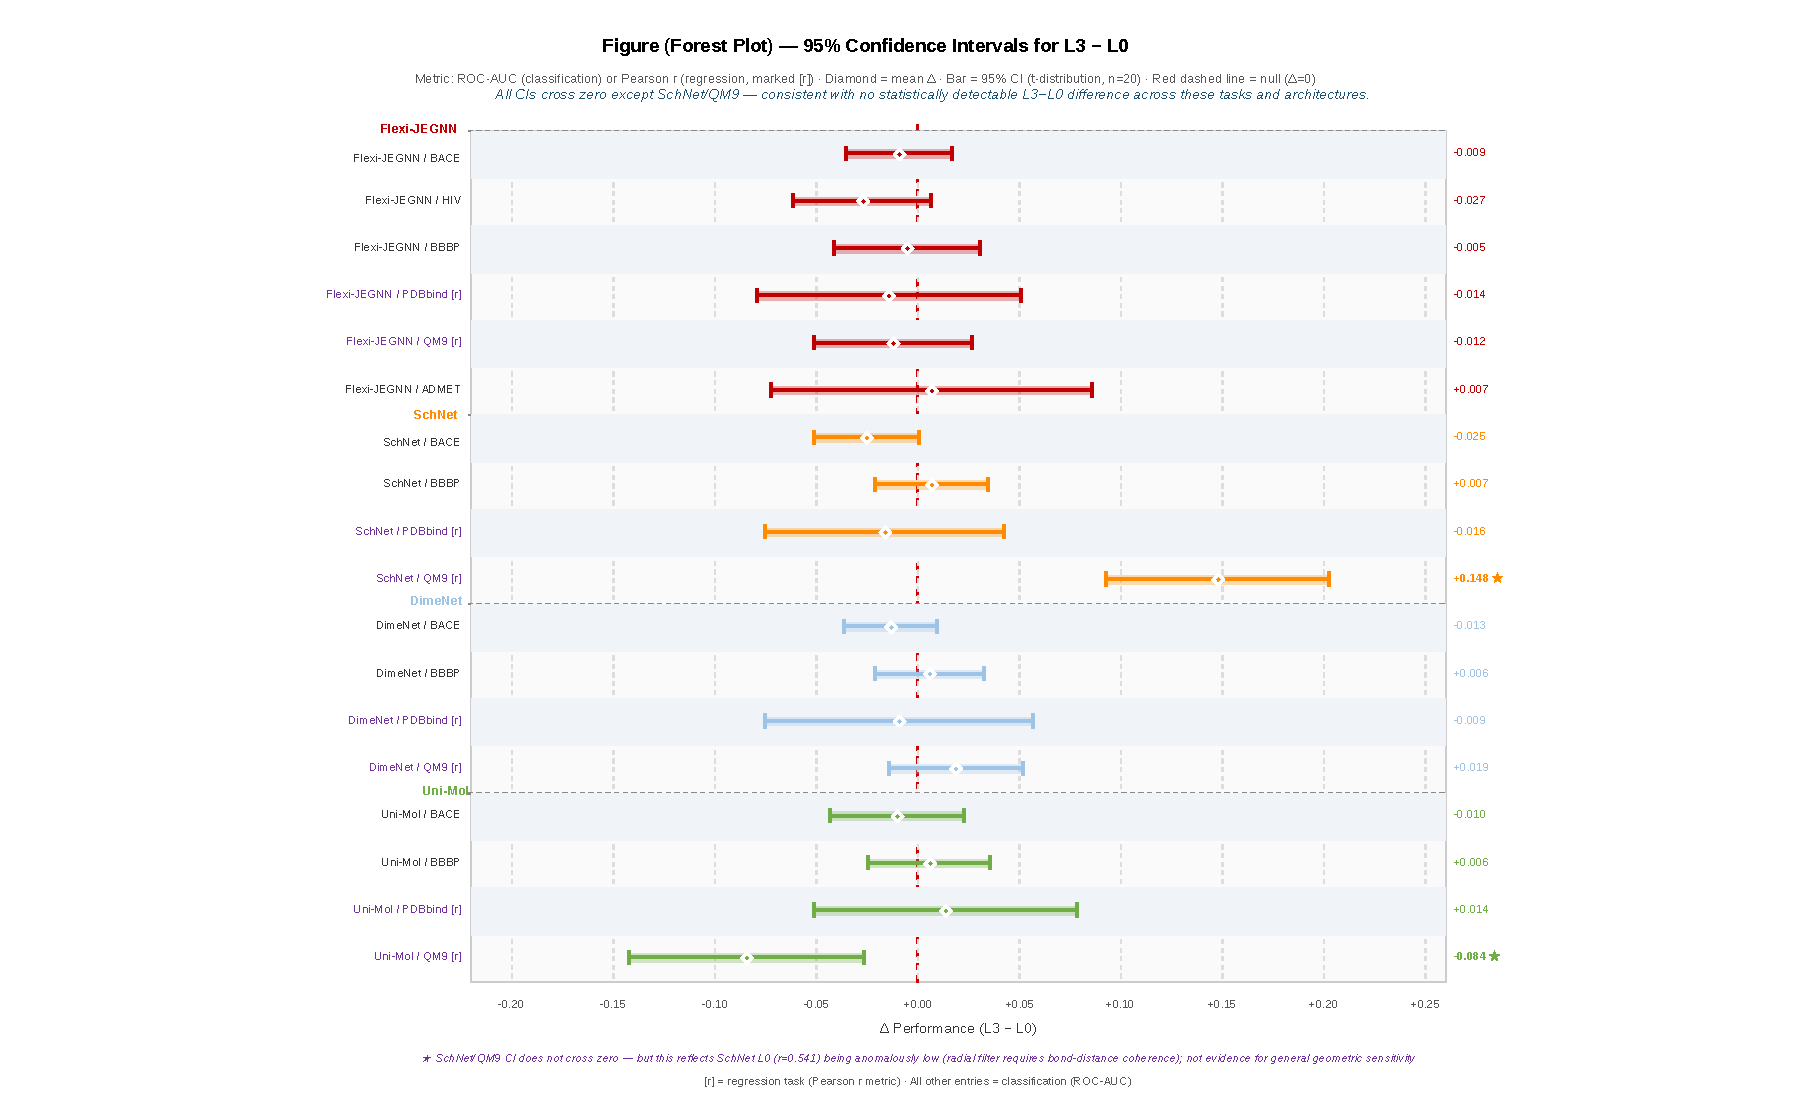
\includegraphics[width=\textwidth]{FigForestPlot.drawio.pdf}
  \caption{Forest plot of the signed performance difference $\Delta = L3 - L0$ (95\% CI, $n{=}20$ seeds)
  for all dataset $\times$ model combinations.  Horizontal bars are 95\% CIs; central markers
  indicate the mean $\Delta$.  All CIs include zero except SchNet/QM9, consistent with no statistically detectable L3$-$L0 difference across the dataset--model
  combinations.  ROC-AUC for classification; Pearson~$r$ for PDBbind and QM9 (regression).}
  \label{fig:forest_plot}
\end{figure}

%% ===========================================================

\bibliography{Refs}

\end{document}